\chapter{Syntactic Metalogic} \label{ch:syntax}

%% TO DO: example -- first-order mereology

%% TO DO: example from Goodman and Quine, about making something true
%% by definition

%% TO DO: What is preserved in Quine-Glymour equivalence?

%% TO DO: do use function symbols in formulation of derivation rules

First-order logic plays a starring role in our best account of the
structure of human knowledge.  There is reason to believe that
first-order logic is fully sufficient to encode \textit{all}
deductively valid reasoning.  It was discovered in the early 20th
century that first-order logic is powerful enough to axiomatize many
of the theories that mathematicians use, such as number theory, group
theory, ring theory, field theory, etc..  And although there are other
mathematical theories that are overtly second-order (e.g.\ the theory
of topological spaces quantifies over subsets, and not just individual
points), nonetheless first-order logic can be used to axiomatize
set-theory, and any second-order theory can be formalized within set
theory.  Thus, first-order logic provides an expansive framework in
which much, if not all, deductively valid human reasoning can be
represented.

In this chapter, we will study the properties of first-order logic,
the theories that can be formulated within it, and the relations that
hold between them.  Let's begin from the concrete --- with examples of
some theories that can be regimented in first-order logic.

\section{Regimenting theories}

%% TO DO: Carnap -- rational reconstruction

%% TODO: Axiomatizations of STR ?? 

\begin{example}[The theory of partial orders] \label{ex:poset} We
  suppose that there is a relation, which we'll denote by $\leq$, and
  we then proceed to lay down some postulates for this relation.  In
  particular:
\begin{itemize}
\item Postulate 1: The relation $\leq$ is reflexive in the sense that
  it holds between anything and itself.  For example, if we were
  working with numbers, we could write $2\leq 2$, or more generally,
  we could write $n\leq n$ for any $n$.  For this last phrase, we have
  a shorthand: we abbreviate it by $\forall n(n\leq n)$, which can be
  read out as, ``for all $n$, $n\leq n$.''  The symbol $\forall$ is
  called the \textbf{universal quantifier}.
\item Postulate 2: The relation $\leq$  is transitive in the sense
  that if $x\leq y$ and $y\leq z$, then $x\leq z$.  Again, we can
  abbreviate this last sentence as
  \[ \forall x\forall y\forall z((x\leq y\wedge y\leq z)\to x\leq z)
    ,\]
  which can be read as, ``for all $x$, for all $y$, and for all $z$,
  if \dots ''
\item Postulate 3: The relation $\leq$ is antisymmetric in the sense
  that if $x\leq y$ and $y\leq x$, then $x=y$.  This postulate can be
  formalized as:
    \[ \forall x\forall y((x\leq y\wedge y\leq x)\to x=y) .\]
  \end{itemize}
  In these previous postulates, we see the same logical connectives
  that we used in propositional logic, such as $\wedge$ and $\to$.
  But now these connectives might hold between things that are not
  themselves sentences.  For example, $x\leq y$ is not itself a
  sentence, because $x$ and $y$ aren't names of things.  We say that
  $x$ and $y$ are \emph{variables}, that $\leq$ is a \emph{relation
    symbol}, and that $x\leq y$ is a \emph{formula}.  Finally, the
  familiar symbol $=$ is also a relation symbol. \end{example}

We've described just the barest of bones of the theory of a partial
order.  There are a couple of further things that we would definitely
like to be able to do with this theory.  First, we would like to be
able to derive consequences from the postulates --- i.e.\ we would
like to derive theorems from the axioms.  In order to do so, we will
need to specify the \textbf{rules of derivation} for first-order
logic.  We will do that later in this chapter.  We would also like to
be able to identify mathematical structures that exemplify the axioms
of partial order.  To that end, we devote the following chapter to the
\textbf{semantics}, or \textbf{model theory}, of first-order logic.

\begin{example}[The theory of a linear order] Take the axioms of the
  theory of a partial order, and then add the following axiom:
  \[ \forall x\forall y((x\leq y)\vee (y\leq x)) .\] This axiom says
  that any two distinct things stand in the relation $\leq$.  In other
  words, the elements from the domain form a total order.  There are
  further specifications that we could then add to the theory of a
  linear order.  For example, we could add an axiom saying that the
  linear order has endpoints.  Conversely, we could add an axiom
  saying that the linear order does not have endpoints.  (Note,
  incidentally, that since either one of those axioms could be added,
  the original theory of linear orders is not complete, i.e.\ it
  leaves at least one sentence undecided.)  We could also add an axiom
  saying that the linear order is dense, i.e.\ that between any two
  elements there is yet another element.  \end{example}

\begin{example}[The theory of an equivalence relation] Let $R$ be a
  binary relation symbol.  The following axioms give the theory of an
  equivalence relation:
  \[ \begin{array}{l l l}
       \text{reflexive} & \vdash \: R(x,x) \\
       \text{symmetric} & \vdash \: R(x,y)\to R(y,x) \\
       \text{transitive} & \vdash \: (R(x,y)\wedge R(y,z))\to
                           R(x,z) \end{array}
                       \] Here when we write an open formula, such as
$R(x,x)$, we mean to implicitly quantify universally over the free variables.  That is,
$\vdash R(x,x)$ is shorthand for $\vdash \forall xR(x,x)$.   \end{example}

%% Perhaps a couple more examples at this point?  e.g. mereology?
%% e.g. group theory

\begin{example}[The theory of abelian groups] We're all familiar with
  number systems such as the integers, the rational numbers, and the
  real numbers.  What do these number systems have in common?  One
  common structure between them is that they have a binary relation
  $+$, a neutral element $0$, and each number has a unique inverse.
  We also notice that the binary relation $+$ is associative in the
  sense that $x+(y+z)=(x+y)+z$, for all $x,y,z$.  We can formalize
  this last statement as
  \[ \forall x\forall y\forall z(x+(y+z)=(x+y)+z) .\] In many familiar
  cases, the operation $+$ is also commutative, that is
  \[ \forall x\forall y(x+y=y+x ) .\] Bringing these postulates
  together, we have the theory of abelian groups.  Notice that in this
  case, we've enlarged our vocabulary to include a symbol $+$ and a
  symbol $0$.  The symbol $+$ is not exactly a relation symbol, but
  instead is a function symbol.  Intuitively speaking, given any names
  $n$ and $m$ of numbers, $n+m$ also names a number.  Similarly, $0$
  is taken to be the name of some specific number, and in this sense
  it differs from variables.
\end{example}

\begin{example}[Boolean algebra] \label{ex:bool} Suppose that $+$ and
  $\cdot$ are binary function symbols, and that $0$ and $1$ are
  constant symbols.  If you look back at our discussion of Boolean
  algebras (Section \ref{sec:bool}), you'll see that each of the
  axioms amounts to a first-order sentence, where we use the $+$
  symbol instead of the $\vee$ symbol, and the $\cdot$ symbol instead
  of the $\wedge$ symbol (since those symbols are already being used
  as our logical connectives).  The theory of Boolean algebras is an
  example of an \emph{algebraic theory}, which means that it can be
  axiomatized using only function symbols and
  equations.  \end{example}

\begin{example}[Arithmetic] It's possible to formulate a first-order
  theory of arithmetic, e.g.\ Peano arithmetic.  For this, we could
  use a signature $\Sigma$ with constant symbols $0$ and $1$, and
  binary function symbols $+$ and $\cdot$.   \end{example}

\begin{example}[Set theory] It's possible to formulate a first-order
  theory of sets, e.g.\ Zermelo-Fraenkel set theory.  For this, we
  could use a signature $\Sigma$ with a single relation symbol $\in$.
  However, for the elementary theory of the category of sets (ETCS),
  as we developed in Chapter \ref{cat-set}, it would be more natural
  to use the framework of many-sorted logic, having one sort for sets,
  and another sort for functions between sets.  For more on
  many-sorted logic, see Chapter \ref{chap-second}.  \end{example}

\begin{example}[Mereology] There are various ways to formulate a
  first-order theory of mereology.  Most presentations begin with a
  relation symbol $pt (x,y)$ to indicate that $x$ is a part of $y$.
  Then we add some axioms that look a lot like the axioms for the
  less-than relation $<$ for a finite Boolean algebra.  \end{example}

\section{Logical grammar}

Abstracting from the previous examples, and many others like them
throughout mathematics, we now define the language of first-order
logic as follows.

\begin{defn} The \textbf{logical vocabulary} consists of the symbols:
  \[ \bot \; \forall \; \exists \; \wedge \; \vee \; \neg \; \to \; (
    \; ) \] The symbol
  $\bot$ will serve as a propositional constant.  The final two
  symbols here, the parentheses, are simply punctuation symbols that
  will allow us to keep track of groupings of the other
  symbols. \end{defn}

Please note that we intentionally excluded the equality symbol $=$
from the list of logical vocabulary.  Several philosophers in the 20th
century discussed the question of whether the axioms for equality were
analytic truths, or whether they should be considered to form a
specific, contingent theory.  We will not enter into the philosophical
discussion at this point, but it will help us to separate out the
theory of equality from the remaining content of our logical system.
We will also take a more careful approach to variables by treating
them as part of a theory's non-logical vocabulary.  Our reason for
doing so will become clear when we discuss the notion of translations
between theories.

\begin{defn} A \textbf{signature} $\Sigma$ consists of:
  \begin{enumerate} \item A countably infinite collection of
    \textbf{variables}.
  \item A collection of \textbf{relation symbols}, each of which is
    assigned a natural number called its \textbf{arity}.  A $0$-ary
    relation symbol is called a \emph{propositional constant}.
  \item A collection of \textbf{function symbols}, each of which is
    assigned a natural number called its arity.  A $0$-ary function
    symbol is called a \emph{constant symbol}. \end{enumerate}
\end{defn}

\begin{disc} Some logicians use the name \emph{similarity type} as a
  synonym for \emph{signature}.  There is also a tendency among
  philosophers to think of a signature as the vocabulary for an
  \emph{uninterpreted language}.  The idea here is that the elements
  of the signature are symbols that receive meaning by means of a
  semantic interpretation.  Nonetheless, we should be careful with
  this kind of usage, which might suggest that formal languages lie on
  the ``mind side'' of the mind--world divide, and that an
  interpretation relates a mental object to an object in the world.
  In fact, formal languages, sentences, and theories are all
  \textit{mathematical objects} --- of precisely the same ontological
  kind as the models that interpret them.  We discuss this issue
  further in the next chapter.   \end{disc}

Although a list of variables is technically part of a signature, we
will frequently omit mention of the variables, and defer to using the
standard list $x,y,x_1,x_2,\dots $.  Only in cases where we are
comparing two theories will we need to carefully distinguish their
variables from each other.

\begin{example} Every propositional signature is a special case of a
  signature in the sense just defined.   \end{example}

\begin{example} For the theory of abelian groups, we used a signature
  $\Sigma$ that has a binary function symbol $+$ and a constant symbol
  $0$.  Some other presentations of the theory of abelian groups use a
  signature $\Sigma '$ that also has a unary function symbol ``$-$''
  for the inverse of an element.  Still other presentations of the
  theory use a signature that doesn't have the constant symbol $0$.
  We will soon see that there is a sense in which these different
  theories all deserve to be called \textit{the} theory of abelian
  groups.  \end{example}

\begin{disc} Let $\Sigma$ be the signature consisting of a binary
  relation symbol $r$, and let $\Sigma '$ be the signature consisting
  of a binary relation symbol $R$.  Are these signatures the same or
  different?  That depends on what implicit background conventions
  that we adopt, in particular, whether our specification of a
  signature is case-sensitive or not.  In fact, we could adopt a
  convention that was even more strict in how it individuates
  signatures.  For example, let $\Sigma ''$ be the signature
  consisting of a binary relation symbol $r$.  One could say that
  $\Sigma ''$ is a different signature from $\Sigma$ because the $r$
  in $\Sigma ''$ occurs at a different location on the page than the
  $r$ that occurs in $\Sigma$.  Of course, we would typically assume
  that $\Sigma ''=\Sigma$, but such a claim depends on an implicit
  background assumption that there is a single letter-form of which
  the two occurences of $r$ are instances.

  We will generally leave these implicit background assumptions
  unmentioned.  Indeed, to make these background assumptions explicit,
  we would have to rely on further implicit background assumptions,
  and we would never make progress in our study of first-order
  logic. 
\end{disc}


Let $\Sigma$ be a fixed signature.  We first define the sets of
$\Sigma$-terms and $\Sigma$-formulas.

\begin{defn} We simultaneously define the set of
  \textbf{$\Sigma$-terms}, and the set $FV(t)$ of \textbf{free
    variables} of a $\Sigma$-term $t$ as follows:
  \begin{enumerate}
  \item If $x$ is a variable of $\Sigma$, then $x$ is a $\Sigma$-term
    and $FV(x)=\{ x\}$.
  \item If $f$ is a function symbol of $\Sigma$, and $t_1,\dots ,t_n$
    are $\Sigma$-terms, then $f(t_1,\dots ,t_n)$ is a $\Sigma$-term
    and
    $$ FV(f(t_1,\dots ,t_n)) \: := \: FV(t_1)\cup\cdots\cup FV(t_n) .$$  \end{enumerate}
\end{defn}

\begin{defn} We simultaneously define the set of
  \textbf{$\Sigma$-formulas}, and the set $FV(\vp )$ of free variables
  of each $\Sigma$-formula $\vp$ as follows:
\begin{enumerate}
\item $\bot$ is a formula and $FV(\bot )=\emptyset$.
\item If $r$ is an $n$-ary relation symbol in $\Sigma$, and
  $t_1,\dots ,t_n$ are terms, then $r(t_1,\dots ,t_n)$ is a formula
  and
  $$ FV(r(t_1,\dots ,t_n)) \: := \: FV(t_1)\cup\cdots\cup FV(t_n) .$$
\item If $\phi$ and $\psi$ are formulas, then $\phi\wedge \psi$ is a
  formula with $FV(\vp\wedge\psi )=FV(\vp )\cup FV(\psi )$.  Similarly
  for the other Boolean connectives $\neg ,\vee,\to$.
\item If $\vp$ is a formula, then so is $\exists x\vp$ and
  $FV(\exists x\vp )=FV(\vp )\backslash \{ x\}$.  Similarly for
  $\forall x\vp$.  \end{enumerate} A formula $\vp$ is called
\emph{closed}, or a \emph{sentence}, if $FV(\vp
)=\emptyset$.  \end{defn}

A more fully precise definition of $\Sigma$-formulas would take into
account the precise location of parentheses.  For example, we would
want to say that $(\vp\wedge \psi )$ is a $\Sigma$-formula when $\vp$
and $\psi$ are $\Sigma$-formulas.  Nonetheless, we will continue to
allow ourselves to omit parentheses when no confusion is likely to
result.

\begin{note} Our definition of the set of formulas allows for
  redundant quantification.  For example, the string
  $\exists x\forall x(x=x)$ is well-formed formula according to our
  definition.  This formula results from applying the quantifier
  $\exists x$ to the sentence $\forall x(x=x)$.  We will have to be
  careful in our definition of derivation rules, and semantic rules,
  to take the case of empty quantification into account.
\end{note}

\begin{defn} The \textbf{elementary formulas} are those of the form
  $r(t_1,\dots ,t_n)$, i.e.\ formulas that involve no Boolean
  connectives or quantifiers. \end{defn}

It is helpful to think of formulas in terms of their \textbf{parse
  trees.}  For example, the formula
$\forall x\exists y(r(x,x)\to r(x,y))$ has the following parse tree:

\bigskip 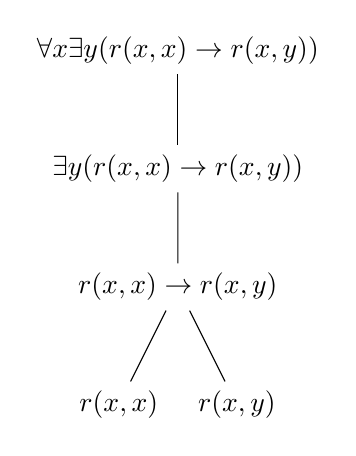
\begin{tikzpicture}[level distance=1.5cm,
  level 1/.style={sibling distance=3cm},
  level 2/.style={sibling distance=1.5cm}]
  \node {$\forall x\exists y(r(x,x)\to r(x,y))$}
    child {node {$\exists y(r(x,x)\to r(x,y))$}
      child {node {$r(x,x)\to r(x,y)$}
        child {node {$r(x,x)$}}
        child {node {$r(x,y)$}}}};
\end{tikzpicture}

\noindent The bottom nodes must each be elementary formulas, i.e.\
either $\bot$, or a relation symbol followed by the appropriate number
of terms.  Each parent-child relationship in the tree corresponds to
one of the Boolean connectives or to one of the quantifiers.

Formulas stand in one-to-one correspondence with parse trees: each
well-formed tree ends with a specific formula, and no other tree
yields the same formula.  Using the identity of formulas and parse
trees, we can easily define a few further helpful notions:

\begin{defn} Let $\vp$ be a $\Sigma$-formula.  The family of
  \textbf{subformulas} of $\vp$ consists of all those formulas that
  occur at some node in its parse tree.  \end{defn}

\begin{defn} If a quantifier $\exists x$ occurs in the formula $\vp$,
  then the \textbf{scope} of that occurrence is the formula which
  occurs at the immediately previous node in the parse
  tree.  \end{defn}

For example, in the formula $\forall x\exists y(r(x,x)\to r(x,y))$,
the scope of $\exists y$ is the formula $r(x,x)\to r(x,y)$.  In
contrast, in the formula $\forall x(r(x,x)\to \exists yr(x,y))$, the
scope of $\exists y$ is the formula $r(x,y)$.

We can now make the notion of free and bound variables even more
precise.  In particular, each individual occurrence of a variable in
$\vp$ is either free or bound.  For example, in the formula
$p(x)\wedge \exists xp(x)$, $x$ occurs freely in the first subformula,
and bound in the second subformula.

\begin{defn}[Free and bound occurrences] An occurence of a variable
  $x$ in $\vp$ is \textbf{bound} just in case that occurrence is
  within the scope of either $\forall x$ or $\exists x$.  Otherwise
  that occurence of $x$ is free. \end{defn}

We could now perform a sanity check to make sure that our two notions
of bound/free variables coincide with each other.

\begin{fact} A variable $x$ is free in $\vp$ (in the sense of the
  definition of $\Sigma$-formulas) if and only if there is a free
  occurence of $x$ in $\vp$ (in the sense that this occurence does not
  lie in the scope of any corresponding quantifier).  \end{fact}


It is also sometimes necessary to distinguish particular occurrences
of a subformula of a formula, and to define the \textbf{depth} at
which such an instance occurs.

\begin{defn} Let $\psi$ be a node in the parse tree of $\vp$.  The
  \textbf{depth} of $\psi$ is the number of steps from $\psi$ to the
  root node.  We say that $\psi$ is a \textbf{proper subformula} of
  $\vp$ if $\psi$ occurs with depth greater than $0$. \end{defn}

The parse trees of formulas are finite, by definition.  Therefore, the
depth of every occurrence of a subformula of $\vp$ is some finite
number.

There are a number of other properties of formulas that are definable
in purely syntactic terms.  For example, we could define the
\textbf{length} of a formula.  We could then note that the connectives
take formulas of a certain length and combine them to create formulas
of a certain greater length.

\begin{exercise} Show that no $\Sigma$-formula can occur as a proper
  subformula of itself. \end{exercise}

% We can give a more precise definition of the structure of a
% $\Sigma$-formula by making use of the notion of a \emph{list} of
% formulas.

% \begin{defn} The family of \emph{lists} of formulas is defined by the
%   following conditions:
%   \begin{enumerate}
%   \item If $\vp _1,\dots ,\vp _n$ are formulas, then
%     $\langle \vp _1 , \cdots , \vp _n\rangle$ is a list.
%   \item If $\sigma _1,\dots ,\sigma _n$ are either formulas or lists
%     of formulas, then $\langle \sigma _1 , \cdots ,\sigma _n\rangle$
%     is a list. \end{enumerate}
% \end{defn}

% A typical list of formulas looks something like this:
% \[ \langle \vp _1 ,\langle \vp _2 ,\vp _1 \rangle ,\vp _3 \rangle .\]
% We are especially interested in lists of formulas such as:
% \[ \langle \vp _1\wedge \vp _2,\langle \vp _1\rangle ,\langle \vp
%   _2\rangle \rangle .\] Here the first item is a Boolean combination,
% the second item is a list with one entry (the first conjunct), and the
% third item is a list with one entry (the second conjunct).

% \begin{defn} Given a list $\sigma$, we let $\sigma _i$ denote the
%   $i$-th entry.  Note that $\sigma _i$ could be another list, or it
%   could be a formula. \end{defn}

% \begin{defn} We define the family of \emph{f-lists} of formulas as
%   follows: \begin{enumerate}
%   \item If $\vp$ is an atomic formula, then $\langle\vp\rangle$ is an
%     f-list.
%   \item If $\sigma$ and $\tau$ are f-lists such that $\sigma _1$ and
%     $\tau _1$ are formulas, then
%     $\langle \sigma _1\wedge \tau _1,\sigma ,\tau \rangle$ is an
%     f-list.
%   \item Similar clauses for the other Boolean connectives.    
%   \item If $\sigma$ is an f-list such that $\sigma _1$ is a formula,
%     then $\langle \forall x\sigma _1 ,\sigma \rangle$ is an f-list.
%   \item A similar clause for $\exists x$.
%   \end{enumerate}
%   \end{defn}

%   \begin{prop} There is a one-to-one correspondence between formulas
%     and f-lists of formulas.  In particular, for each formula $\vp$,
%     there is a unique f-list $\sigma$ such that $\sigma
%     _1=\vp$. \end{prop}

%   \begin{proof} Define a function $f$ from formulas to f-lists
%     by: \begin{enumerate}
%     \item $f(\vp )=\langle\vp\rangle$ for $\vp$ atomic.
%     \item
%       $f(\vp\wedge\psi )=\langle\vp\wedge\psi,f(\vp ),f(\psi
%       )\rangle$, and similarly for the other Boolean connectives.
%     \item $f(\forall x\vp)=\langle\forall x\vp ,f(\vp )\rangle$, and
%       similarly for $\exists x\vp$.
%     \end{enumerate}
%     Then $f(\vp )_1=\vp$, from which it follows that $f$ is injective.

%     We now show that $f$ is surjective, by induction on the
%     construction of f-lists.  Base case: if
%     $\sigma =\langle \vp\rangle$, for $\vp$ an atomic formula, then
%     $\sigma =f(\vp )$.

%         Inductive step: assume that
%         $\sigma = \langle \vp\wedge\vp ',\tau ,\tau '\rangle$, where
%         $\tau$ and $\tau '$ are f-lists in the image of the function
%         $f$.  Let $\tau$ and $\tau '$ be formulas such that
%         $\tau =f(\theta )$ and $\tau '=f(\theta ')$.  By the
%         definition of $f$, $\tau _1=\theta$ and $\tau '_1=\theta '$.
%         By the definition of f-lists, $\vp = \tau _1$ and
%         $\vp '=\tau '_1$.  Thus, $\theta =\vp$ and $\theta '=\vp '$,
%         from which it follows that
%         \[ \sigma \:=\: \langle \vp\wedge\vp',f(\vp ),f(\vp ')\rangle
%           \:=\: f(\vp\wedge \vp ') .\] The remaining inductive steps
%         are similar, and we leave them to the reader.  \end{proof}

%       \begin{disc} In any f-list
%         $\sigma = \langle \vp ,\dots \rangle$, the angle brackets are
%         balanced.  What's more, any formula $\psi$ that occurs in
%         $\sigma$ is surrounded by $n$ pairs $\langle\cdot\rangle$, for
%         some $n\geq 1$.  Then $n-1$ is the \emph{depth} of this
%         occurence of $\psi$ in $\vp$. \end{disc}





% %% Example proofs by induction on construction?

%       [[TO DO: move]] Any time we define a set inductively, we have a
%       corresponding method of proof by induction.  In this case, we
%       can prove that a property $\mathbb{P}$ holds for all
%       $\Sigma$-formulas by showing that $\mathbb{P}$ holds for all
%       elementary $\Sigma$-formulas, and that $\mathbb{P}$ is preserved
%       by the various operations that allow us to construct more
%       complex $\Sigma$-formulas.  What is a bit more difficult in this
%       case is proving that some property holds of all
%       $\Sigma$-sentences, when that property does not hold of all
%       $\Sigma$-formulas.  In such cases, we'll have to look for a
%       clever way to modify the standard sort of proof by induction.


%% TO DO: define the notation $\vp [t/x]$

We now define a substitution operation $\vp\mapsto \vp [t/x]$ on
formulas, where $t$ is a fixed term, and $x$ is a fixed variable.  The
intention here is that $\vp [t/x]$ results from replacing all free
occurrences of $x$ in $\vp$ with $t$.  We first define a corresponding
operation on terms.

\begin{defn} Let $t$ be a fixed term, and let $x$ be a fixed variable.
  We define the operation $s\mapsto s[t/x]$, where $s$ is an arbitrary
  term, as follows:
  \begin{enumerate}
  \item If $s$ is a variable, then $s[t/x]\equiv s$ when
    $s\not\equiv x$, and $s[t/x]\equiv t$ when $s\equiv x$.  (Here
    $\equiv$ means literal identity of strings of symbols.)
  \item Suppose that $s\equiv f(t_1,\dots ,t_n)$, where $f$ is a function
    symbol and $t_1,\dots ,t_n$ are terms.  Then we define 
    \[ s[t/x] \: \equiv \: f(t_1[t/x],\dots ,t_n[t/x]) .\] This
    includes the special case where $f$ is a $0$-ary function symbol,
    where $f[t/x]\equiv f$.
  \end{enumerate}
\end{defn}

\begin{defn} Let $t$ be a fixed term, and let $x$ be a fixed variable.
  We define the operation $\vp\mapsto \vp [t/x]$, for $\vp$ an
  arbitrary formula, as follows:
  \begin{enumerate}
  \item For the proposition $\bot$, let $\bot [t/x]:=\bot$.
  \item For an elementary formula $r(t_1,\dots ,t_n)$, let 
    \[ r(t_1,\dots ,t_n)[t/x] \: := \: r(t_1[t/x],\dots ,t_n[t/x]) .\]
  \item For a Boolean combination $\vp\wedge\psi$, let
    \[ (\vp\wedge\psi )[t/x] \: : = \: \vp [t/x]\wedge \psi [t/x] ,\]
    and similarly for the other Boolean connectives.
  \item For an existentially quantified formula $\exists y\vp$, let
    \[ (\exists y\vp )[t/x] := \left\{ \begin{array}{l l} \exists y(\vp
                                         [t/x]) & \text{if}\; x\not\equiv y , \\
                                         \exists y\vp & \text{if}\;
                                                        x\equiv y
                                                        .\end{array}
                                                    \right. \]
\item For a universally quantifier formula $\forall y\vp$, let \[ (\forall y\vp )[t/x] := \left\{ \begin{array}{l l}
                                                  \forall y(\vp
                                         [t/x]) & \text{if}\; x\not\equiv y , \\
                                         \forall y\vp & \text{if}\;
                                                        x\equiv y
                                                        .\end{array}
                                                    \right. \]
                                                  
\end{enumerate}
\end{defn}

\begin{prop} For any formula $\vp$, the variable $x$ is not free in
  $\vp [y/x]$. \end{prop}

\begin{proof} We first show that $x\not\in FV(t[y/x])$ for any term
  $t$.  That result follows by a simple induction on the construction
  of terms.

  Now let $\vp$ be an elementary formula.  That is,
  $\vp =r(t_1,\dots ,t_n)$.  Then we have
  \[ \begin{array}{l l l} FV(\vp [y/x]) & = & FV(r(t_1,\dots ,t_n)[y/x]) \\
                                        &=& FV(r(t_1[y/x],\dots ,t_n[y/x])) \\
                                        &=& FV(t_1[y/x])\cup\cdots\cup
                                            FV(t_n[y/x])
                                            .\end{array} \] %%
                                        Since $x\not\in FV(t_i[y/x])$,
                                        for $i=1,\dots ,n$, it follows
                                        that $x\not\in FV(\vp [y/x])$.

The argument for the Boolean connectives is trivial, so we turn to the
argument for the quantifiers.  Suppose that the result is true for
$\vp$.  We need to show that it's also true for $\exists v\vp$.
Suppose first that $v\equiv x$.  In this case we have
\[ (\exists v\vp )[y/x] = (\exists x\vp )[y/x] = \exists x\vp .\]
Since $x\not\in FV(\exists x\vp )$, it follows that $x\not\in
FV((\exists v \vp )[y/x])$.  Suppose now that $v\not\equiv x$.  In
this case we have
\[ (\exists v\vp )[y/x] = \exists v(\vp [y/x]) .\] Since
$x\not\in FV(\vp [y/x])$, it follows then that
$x\not\in FV((\exists v\vp )[y/x])$. The argument is analogous for the
quantifier $\forall v$.  Therefore, for any formula $\vp$, the
variable $x$ is not free in $\vp [y/x]$.
\end{proof}




%% Things still to prove

%% 1. Substitution in the formula
%% \vp \vdash \psi -- can switch out the free variables

%% 2. Alpha equivalence





\section{Deduction rules}

We suppose again that $\Sigma$ is a fixed signature.  The goal now is
to define a relation $\Gamma \vdash \vp$ of derivability, where
$\Gamma$ is a finite sequence of $\Sigma$-formulas, and $\vp$ is a
$\Sigma$-formula.  Our derivation rules come in three groupings: rules
for the Boolean connectives, rules for the $\bot$ symbol, and rules
for the quantifiers.

\subsection*{Boolean connectives}

We carry over all of the rules for the Boolean connectives from
propositional logic (see Section \ref{sec:pt}).  These rules require
no special handling of variables.  For example, the following is a
valid instance of $\wedge$-elim:
\[ \begin{array}{l}
     \Gamma \RA \vp (x)\wedge \psi (y) \\
     \hline \Gamma \RA \vp (x) \end{array} \]

\subsection*{Falsum} 

We intend for the propositional constant $\bot$ to serve as shorthand
for ``the false.''  To this end, we define its introduction and
elimination rules as follows.

\bigskip \begin{tabular}{c c c } \begin{tabular}{|l l |} \hline \textbf{$\bot$ intro}
    & \begin{tabular}{l}
        $\Gamma \RA \vp\wedge \neg \vp$ \\
        \hline $\Gamma \RA \bot $ \end{tabular} \\
                    \hline \end{tabular}
& & \begin{tabular}{|l l |} \hline  \textbf{$\bot$ elim} & \begin{tabular}{l}
                                             $\Gamma \RA \bot $  \\
                                             \hline $\Gamma \RA \vp
                                             $ \end{tabular} \\
                    \hline \end{tabular} \end{tabular}



\subsection*{Quantifiers}

In order to formulate good derivation rules for the quantifiers, we
have to make a couple of strategic choices.  In actual mathematical
practice, mathematicians simply introduce new vocabulary whenever they
need it.  In some cases, new vocabulary is introduced by way of
definition --- for example, when a mathematician says something like,
``we say that a number $x$ is \textit{prime} just in case \dots '',
where the words following the dots refer to previously understood
mathematical concepts.  In other cases, the newly introduced
vocabulary is really just newly introduced notation --- for example,
when a mathematician says something like, ``let $n$ be a natural
number.''  In this latter case, the letter ``$n$'' wasn't a part of
the original vocabulary of the theory of arithmetic, and was
introduced as a matter of notational convenience.

Nonetheless, for our purposes it will be most convenient to have a
fixed vocabulary $\Sigma$ for a theory.  But this means that if
$\Sigma$ has no constant symbols, then we might have trouble making
use of the quantifier introduction and elimination rules.  For
example, imagine trying to derive a theorem in the theory of Boolean
algebras is you weren't permitted to say, ``let $a$ be an arbitrary
element of the Boolean algebra $B$.''  In order to simulate
mathematics' free use of new notation, we'll simply be a bit more
liberal in the way that we allow free variables to be used.  To this
end, we define the following notion:

\begin{defn} We say that \emph{$t$ is free for $x$ in $\vp$} just in
  case one of the following conditions holds:
  \begin{enumerate}
  \item $\vp$ is atomic, or
  \item $\vp$ is a Boolean combination of formulas, in each of which
    $t$ is free for $x$, or
  \item $\vp:=\exists y\psi$, and $y\not\in FV(t)$, and $t$ is free
    for $x$ in $\psi$, where $x\neq y$. \end{enumerate} \end{defn}

Intuitively speaking, $t$ is free for $x$ in $\vp$ just in case
substituting $t$ in for $x$ in $\vp$ does not result in any of the
variables in $t$ being captured by quantifiers.  For example, in the
formula $p(x)$, the variable $y$ is free for $x$ (since $y$ is free in
$p(y)$).  In contrast, in the formula $\exists yp(x)$, the variable
$y$ is not free for $x$ (since $y$ is not free in $\exists yp(y)$).
We will need this notion in order to coordinate our intro and elim
rules for the quantifiers.  For example, the rule of $\forall$-elim
should say something like: $\forall x\vp (x)\vdash \vp (y)$.  However,
if this rule were not restricted in some way, then it would yield
\[ \forall x\exists y(x\neq y) \: \vdash \: \exists y(y\neq y) ,\]
which is intuitively invalid.

\begin{figure}[H]
\begin{tabular}{|l l l|}
  \hline  \textbf{$\forall$ intro}
  & \makecell[l]{ $\Gamma \: \vdash \:
    \vp$ \\ \hline $\Gamma \: \vdash \: \forall x\vp$ }
  & \makecell[l]{\small where $x$ is not free in $\Gamma$.}  \\ \hline \end{tabular}

\bigskip \begin{tabular}{|l l l|} \hline 
  \textbf{$\forall$ elim} & \makecell[l]{
                            $\Gamma \: \vdash \: \forall x\vp$ \\ \hline
  $\Gamma \: \vdash \: \vp [t/x]$ } & \makecell[l]{\small where $t$
                                      is free for $x$.} \\ \hline
\end{tabular} \end{figure}

The $\forall$-intro rule is easy to apply, for we only need to check
that the variable $x$ doesn't occur in the assumptions $\Gamma$ from
which $\vp$ is derived.  Note that application of the $\forall$-intro
rule can result in empty quantification; so example,
$\forall x\forall xp(x)$ follows from $\forall xp(x)$.

To understand the restrictions on $\forall$-elim, note that it does
license
\[ \forall x\, r(x,x) \: \vdash \: r(y,y) , \]
since $r(x,x)[y/x]\equiv r(y,y)$.  In contrast, $\forall$-elim does not license
\[ \forall x\,r(x,x) \: \vdash \: r(x,y) , \] since it is not the case
that $r(x,x)[y/x]\equiv r(x,y)$.  Similarly, $\forall$-elim does not
license
\[ \forall x\exists y\,r(x,y) \: \vdash \: \exists y\,r(y,y) ,\] since
$y$ is not free for $x$ in $\exists y\,r(x,y)$.  Finally,
$\forall$-elim permits universal quantifiers to be peeled off when
they don't bind any variables.  For example, $\forall x\,p\vdash p$ is
licensed by $\forall$-elim.

Now we turn to the rules for the existential quantifier.  First we
state the rules in all their sequential glory:

\begin{figure}[H]
  \begin{tabular}{|l l l|} \hline \textbf{$\exists$ intro} &
    \makecell[l]{ $\Gamma \: \vdash \: \vp [t/x]$ \\ \hline
      $\Gamma \: \vdash \: \exists x\vp $ } & \makecell[l]{\small
      provided $t$ is
                                              free for $x$ in $\vp$.} \\
                                              \hline \end{tabular}

\bigskip \begin{tabular}{|l l l|} \hline 
    \textbf{$\exists$ elim} & \makecell[l]{
                             $\Gamma ,\vp \:\vdash \: \psi $ \\
    \hline $\Gamma ,\exists x\vp \: \vdash \: \psi$ } &
                                                        \makecell[l]{\small
                                                        provided $x$
                                                        is not free in
                                                        $\psi$ or
                                                        $\Gamma$.}  \\
    \hline \end{tabular} \end{figure}

If we omit the use of auxiliary assumptions, we can rewrite the
$\exists$ rules as follows:

\begin{figure}[H]
  \begin{tabular}{|l l l|} \hline \textbf{$\exists$ intro} &
\makecell[l]{ $\vdash \: \vp [t/x]$ \\ \hline
      $\vdash \: \exists x\vp $ } & {\small
                                                    provided $t$ is
                                                      free for $x$ in $\vp$.}
    \\ \hline \end{tabular}

\bigskip \begin{tabular}{|l l l|} \hline 
\textbf{$\exists$ elim} & \makecell[l]{
                              $\vp \:\vdash \: \psi $ \\
    \hline $\exists x\vp \: \vdash \: \psi$ } &
                                                            \makecell[l]{\small
                                                            provided $x$
                                                            is not
                                                            free in
                                                            $\psi$.}
    \\ \hline \end{tabular} \end{figure}

Again, let's look at some examples to illustrate the restrictions.
First, in the case of the $\exists$-intro rule, suppose that there
were no restriction on the term $t$.  Let $\vp$ be the formula
$\forall y\,r(x,y)$, and let $t$ be the variable $y$, in which case
$\vp [t/x]\equiv \forall y\,r(y,y)$.  Then the $\exists$-in rule would
yield
\[ \forall y\,r(y,y) \: \vdash \: \exists x\forall y\,r(x,y ), \]
which is intuitively invalid.  (Consider, for example, the case where
$r$ is the relation $\leq$ on integers.)  The problem, of course, is
that the variable $y$ is captured by the quantifier $\forall y$ when
substituted into $\vp$.  Similarly, in the case of the $\exists$-elim
rule, if there were no restriction on the variable $x$, then we could
derive $\vp$ from $\exists x\vp$, and then using $\forall$-intro, we
could derive $\exists x\vp\vdash \forall x\vp$.

\subsection*{Structural rules}

In any proof system, there are some more or less tacit rules that
arise from how the system is set up.  For example, when someone learns
natural deduction, e.g.\ via the system presented in Lemmon's {\it
  Beginning Logic}, then she will tacitly assume that she's allowed to
absorb dependencies, e.g.\ if $\phi ,\phi\vdash \psi$ then
$\phi \vdash \psi$.  These more or less tacit rules are called
\emph{structural rules} of the system --- and there is a lot of
interesting research on logical systems that drop one or more of these
structural rules \cite[see][]{restall}.  In this book, we stay within
the confines of classical first-order logic; and we will not need to
be explicit about the structural rules, except for the rule of
\emph{cut}, which allows sequents to be combined.  Loosely speaking,
cut says that if you have sequents $\Gamma \vdash \phi$ and
$\Delta ,\phi\vdash \psi$, then you may derive the sequent
$\Gamma ,\Delta \vdash \psi$.

As was the case with propositional logic, we will not specify a
canonical way of writing predicate logic proofs.  After all, our goal
here is not to teach you the art of logical deduction; rather, our
goal is to reflect on the relations between theories in formal logic.


\subsection*{Equality}

As we mentioned before, there's something of a philosophical debate
about whether the equality symbol $=$ should be considered as part of
the logical or the non-logical vocabulary of a theory.  We don't want
to get tangled up in that argument, but we do wish to point out how
the axioms for equality compare to the axioms for a generic
equivalence relation.

It is typical to write down two axioms for equality, an introduction
and an elimination rule.  Equality introduction permits $\vdash t=t$
with any term $t$.  Equality elimination permits
\[ \begin{array}{c c} t=s \quad \vp [t/s] \\ \hline \vp
   \end{array} \] so long as $t$ is free for $s$ in $\vp$.  Note that equality elimination allows us to
 replace single instances of a term.  For example, if we let $\vp$
 be the formula $r(s,t)$, then $\vp [t/s]$ is the formula $r(t,t)$.
 Hence from $t=s$ and $r(t,t)$, equality elimination permits us to
 derive $r(s,t)$.

 From the equality axioms, we can easily show that it's an equivalence
 relation.  The introducton rule shows that it's reflexive.  For
 symmetry, we let $\vp$ be the formula $y=x$, in which case
 $\vp [x/y]$ is the formula $x=x$.  Thus, we have
   \[ \begin{array}{c c} x=y\quad x=x \\ \hline y=x \end{array} \]
   For transitivity, let $\vp$ be the formula $x=z$, in which case
   $\vp [y/x]$ is the formula $y=z$.  Thus, we have
   \[ \begin{array}{c c} y=x\quad y=z \\ \hline x=z \end{array} \]

   This completes the list of the proof rules for our system of
   first-order logic, i.e.\ our definition of the relation $\vdash$.
   Before proceeding to investigate the properties of this relation,
   let's see a couple of examples of informal proofs.

   \begin{example} Let's show that
     $\exists x(\vp (x)\wedge \psi (x))\vdash \exists x\vp (x)$.
     First note that $\vp (x)\wedge \psi (x)\vdash \vp (x)$ from
     $\wedge$-elim.  Then
     $\vp (x)\wedge \psi (x)\vdash \exists x\vp (x)$ from
     $\exists$-intro.  Finally, since $\exists x\vp (x)$ contains no
     free occurrences of $x$, we have
     $\exists x(\vp (x)\wedge \psi (x))\vdash \exists x\vp
     (x)$.  \end{example}

   \begin{example} Of course we should have
     $\forall x\vp \vdash \forall y(\vp [y/x])$, so long as $y$ is
     free for $x$ in $\vp$.  Using the rules we have, we can derive
     this result in two steps.  First, we have
     $\forall x\vp (x)\vdash \vp [y/x]$ from $\forall$-elim, and then
     $\vp [y/x]\vdash \forall y\vp [y/x]$ by $\forall$-intro.  We only
     need to verify that $x$ is not free in $\vp [y/x]$.  This can be
     shown by a simple inductive argument.   \end{example}

% \begin{prop} For any formula $\vp$, the variable $x$ is not free in
%   $\vp [y/x]$. \end{prop}

% \begin{proof} We first show that $x\not\in FV(t[y/x])$ for any term
%   $t$.  That result follows by a simple induction on the construction
%   of terms.

%   Now let $\vp$ be an elementary formula.  That is,
%   $\vp =r(t_1,\dots ,t_n)$.  Then we have
%   \[ \begin{array}{l l l} FV(\vp [y/x]) & = & FV(r(t_1,\dots ,t_n)[y/x]) \\
%                                         &=& FV(r(t_1[y/x],\dots ,t_n[y/x])) \\
%                                         &=& FV(t_1[y/x])\cup\cdots\cup
%                                             FV(t_n[y/x])
%                                             .\end{array} \] %%
%                                         Since $x\not\in FV(t_i[y/x])$,
%                                         for $i=1,\dots ,n$, it follows
%                                         that $x\not\in FV(\vp [y/x])$.

% The argument for the Boolean connectives is trivial, so we turn to the
% argument for the quantifiers.  Suppose that the result is true for
% $\vp$.  We need to show that it's also true for $\exists v\vp$.
% Suppose first that $v\equiv x$.  In this case we have
% \[ (\exists v\vp )[y/x] = (\exists x\vp )[y/x] = \exists x\vp .\]
% Since $x\not\in FV(\exists x\vp )$, it follows that $x\not\in
% FV((\exists v \vp )[y/x])$.  Suppose now that $v\not\equiv x$.  In
% this case we have
% \[ (\exists v\vp )[y/x] = \exists v(\vp [y/x]) .\] Since
% $x\not\in FV(\vp [y/x])$, it follows then that
% $x\not\in FV((\exists v\vp )[y/x])$. The argument is analogous for the
% quantifier $\forall v$.  Therefore, for any formula $\vp$, the
% variable $x$ is not free in $\vp [y/x]$.
% \end{proof}


%% TO DO: talk about Tarski point -- that theories aren't closed just
%% under deduction, but also conceptually, i.e. by taking definitions
%% TO DO: a philosophical reflection on definition

Recall that propositional logic is compositional in the following
sense: Suppose that $\vp$ is a formula, and $\psi$ is a subformula of
$\vp$.  Let $\vp '$ denote the result of replacing $\psi$ in $\vp$
with another formula $\psi '$ where
$\vdash \psi\leftrightarrow \psi '$.  Then
$\vdash \vp\leftrightarrow \vp '$.  That result is fairy easy to prove
by induction on the construction of proofs.  It also follows from the
truth-functionality of the Boolean connectives, by means of the
completeness theorem.  In this section, we are going to prove an
analogous result for predicate logic.  To simplify notation, we
introduce the following:

\begin{defn} For formulas $\vp$ and $\psi$, we say that $\vp$ and
  $\psi$ are \emph{logically equivalent}, written $\vp\simeq\psi$,
  just in case both $\vp\vdash\psi$ and $\psi\vdash\vp$.
\end{defn}

It is not hard to show that $\simeq$ is an equivalence relation on the
set of formulas.  Note that formulas $\vp$ and $\psi$ can be
equivalent in this sense even if they don't share all free variables
in common --- as long as the non-matching variables occur vacuously.
For example, $p(x)$ is equivalent to $p(x)\wedge (y=y)$, and it's also
equivalent to $p(x)\vee (y\neq y)$.  [The issue here has nothing in
particular to do with the equality relation.  The variable $y$ also
occurs vacuously in $p(y)\vee \neg p(y)$.]  In contrast, the formulas
$p(x)$ and $p(y)$ are not equivalent (in the empty theory), since it's
not universally valid that
$\vdash \forall x\forall y(p(x)\leftrightarrow p(y))$.

\begin{lemma} The relation $\simeq$ is compatible with the Boolean
  connectives in the following sense: if $\phi\simeq\phi '$ and
  $\psi\simeq \psi '$, then
  $(\phi\wedge \psi )\simeq (\phi '\wedge \psi ')$, and similarly for
  the other Boolean connectives. \end{lemma}

The proof of this lemma is a fairly simple application of the
introduction and elimination rules for the connectives.  To complete
the proof of the replacement theorem, we need one more lemma.

\begin{lemma} If $\vp\simeq \psi$ then
  $\exists x\vp\simeq \exists x\psi$. \end{lemma}

\begin{proof} Suppose that $\vp\simeq\psi$, which means that
  $\vp\vdash \psi$ and $\psi\vdash \vp$.  We're now going to show that
  $\exists x\vp\vdash\exists x\psi$.  By $\exists$-in we have
  $\psi\vdash \exists x\psi$, hence by cut we have
  $\vp\vdash\exists x\psi$.  Since $x$ does not occur free in
  $\exists x\psi$, we have $\exists \vp\vdash \exists x\psi$ by
  $\exists$-out.  \end{proof}

%% TO DO: fix this
\begin{thm}[Replacement] Suppose that $\vp$ is a formula in which
  $\psi$ occurs as a subformula, and $\vp '$ is the result of
  replacing $\psi$ with $\psi '$.  If $\psi \simeq \psi '$ then
  $\vp \simeq \vp '$.
\end{thm}

In most presentations of the predicate calculus (i.e.\ the definition
of the relation $\vdash$) the two central results are the soundness
and completeness theorems.  Intuitively speaking, the soundness
theorem shows that the definition doesn't overgenerate, and the
completeness theorem shows that it doesn't undergenerate.  However, in
fact, these results show something quite different --- they show that
the definition of $\vdash$ matches the definition of another relation
$\vDash$.  We will discuss this other relation $\vDash$ in Chapter
\ref{chap-sem}, where we will also prove the traditional soundness and
completeness theorems.  In the remainder of this section, we show that
the predicate calculus is consistent in the following purely syntactic
sense.

\begin{defn} We say that the relation $\vdash$ is \emph{consistent}
  just in case there is some formula $\phi$ that is not provable.
  Similarly, we say that a theory $T$ is \emph{consistent} just in
  case there is a formula $\phi$ such that
  $T\not\vdash\phi$. \end{defn}

Note that the definition of consistency for $\vdash$ presupposes a
fixed background signature $\Sigma$.

\begin{prop} A theory $T$ is consistent iff
  $T\not\vdash\bot$.  \end{prop}

\begin{proof} If $T$ is inconsistent then $T\vdash\phi$ for all
  formulas $\phi$.  In particular, $T\vdash \bot$.  Conversely, if
  $T\vdash\bot$, then RA and DN yield $T\vdash\phi$ for any formula
  $\phi$. \end{proof}

%% TO DO: here I should have the van Dalen proof

\begin{thm} The predicate calculus is consistent. \end{thm}

%% TO DO: I would like to inspect this theorem more closely.  
\begin{proof} Let $\Sigma$ be a fixed predicate logic signature, and
  let $\Sigma '$ be a propositional signature whose cardinality is
  greater than or equal to that of $\Sigma$.  We will use the symbol
  $\vdash ^*$ to denote derivability in the propositional calculus.
  Define a map $\vp\mapsto\vp ^*$ from the formulas of $\Sigma$ to the
  formulas of $\Sigma '$ as follows:
\begin{itemize}
\item $\bot ^*=\bot$
\item For any terms $t_1,\dots ,t_n$,
  $(p_i(t_1,\dots ,t_{n_i}))^*=q_i$.
\item $(\vp\wedge\psi )^*=\vp ^*\wedge \psi ^*$, and similarly for the
  other Boolean connectives.
\item $(\forall x\vp )^*=\vp ^*$ and $(\exists x\vp )^*=\vp ^*$.
\end{itemize}
We now use induction on the definition of $\vdash$ to show that if
$\Gamma\vdash\vp$ then $\Gamma ^*\vdash ^*\vp ^*$.  We will provide a
few representative steps, and leave it to the reader to supply the
others.

\begin{itemize}
\item The base case, rule of assumptions, is trivial.
\item Consider the case of $\wedge$-out.  Suppose that
  $\Gamma\vdash\vp$ follows from $\Gamma\vdash\vp\wedge\psi$ by
  $\wedge$-out.  By the inductive hypothesis,
  $\Gamma ^*\vdash ^*(\vp\wedge\psi )^*$.  Using the definition of
  $(\vp\wedge\psi )^*$, it follows that
  $\Gamma ^*\vdash ^*\vp ^*\wedge \psi ^*$.  Hence by $\wedge$-out, we
  have $\Gamma ^*\vdash ^* \vp ^*$.
\item Consider the case of $\forall$-in.  That is, suppose that
  $\Gamma\vdash\forall x\vp$ is derived from $\Gamma\vdash\vp$ using
  $\forall$-in.  In this case, the induction hypothesis tells us that
  $\Gamma ^*\vdash ^*\vp ^*$.  And since $(\forall x\vp )^*=\vp ^*$,
  we have $\Gamma ^*\vdash ^*(\forall x\vp )^*$.
\end{itemize}
Completing the previous steps shows that if $\Gamma\vdash\vp$ then
$\Gamma ^*\vdash ^*\vp ^*$.  Since the propositional calculus is
consistent, $\not\vdash ^*\bot$, and therefore
$\not\vdash\bot$. \end{proof}

\begin{disc} Notice that the previous proof does not use the fact that
  our $\forall$-intro rule demands that $x$ not occur free in
  $\Gamma$.  Thus, this proof also shows the consistency of a proof
  system with an \textit{unrestricted} $\forall$-in rule.

  But an unrestricted $\forall$-intro rule would nonetheless severely
  restrict the expressive power of our logic.  Indeed, it would
  license
  \[ x\neq y \: \vdash \: \forall y(x\neq y) \: \vdash \: x\neq x , \]
  the last of which contradicts the axioms for equality.  Thus, an
  unrestricted $\forall$-intro would make $\forall x\forall y(x=y)$ a
  tautology. 
\end{disc}





\section{Empirical theories} \label{sec:et}

%% TO DO: Carnap's various attempts to connect theoretical terms with
%% observation language

%% TO DO: here is place to discuss question of whether FOL is too
%% restrictive.  versus "theories in the wild".

%% original Carnap proposal .... and how it was eviscerated by van
%% Fraassen etc.

Here we use the phrase ``empirical theory'' or ``scientific theory'',
to mean a theory that one intends to describe the physical world.  You
know many examples of such theories: Newtonian mechanics, Einstein's
general theory of relativity, quantum mechanics, evolutionary biology,
the phlogiston theory of combustion, etc..  You may also know many
examples of theories from pure mathematics, such as set theory, group
theory, ring theory, topology, and the theory of smooth manifolds.
Intuitively, empirical theories differ in some important way from pure
mathematical theories.  We stress ``intuitively'' here because Quine
brought into question the idea that there is a principled distinction
between two types of theories.  For the time being, we won't engage
directly with Quine's more philosophical arguments against this
distinction.  Instead, we will turn back the clock to the time when
Rudolf Carnap, among others, hoped that formal logic might illuminate
the structure of scientific theories.

Rudolf Carnap was the primary advocate of the idea that philosophers
ought to pursue a {\it syntactic} analysis of scientific theories.
The story is typically told as follows: Carnap sought to construct a
theory {\it of} scientific theories.  Moreover, following in the
footsteps of Bertrand Russell and Gottlob Frege, Carnap believed that
philosophy had no business directly engaging in empirical questions.
As \cite{russ} had argued, philosophers ought to leave empirical
questions to the empirical sciences.  Thus, Carnap thought that a good
philosophical theory of scientific theories ought to restrict itself
to the purely formal aspects of those theories.  In particular, the
``metascientist'', i.e.\ the philosopher of science, ought to make use
only of syntactic concepts.

Carnap begins his {\it Wissenschaftslogik} program in earnest in his
first major book, {\it Logische Aufbau der Welt}.  Already here we see
the emphasis on ``explication'', i.e.\ of taking an intuitive concept,
and providing a precise formal counterpart.  Carnap's paradigms of
explication are those from 19th and early 20th century mathematics ---
explications of concepts such as ``infinity'' and ``continuous
function'' and ``open subset''.  Nonetheless, in the {\it Aufbau},
Carnap hasn't yet found his primary tool of analysis.  That would only
come from the development, in the 1920s, of logical metatheory.
Carnap was working at the time in Vienna, among the other members of
the infamous Vienna Circle.  One of the youngest members of the circle
was Kurt G{\"o}del, whose 1929 PhD thesis contained the first proof of
the completeness of the predicate calculus.  Thus, logical metatheory
--- or metamathematics --- was in the air in Vienna, and Carnap was to
try his hand at applying an analogous methodology to the empirical
sciences.  As the goal of metamathematics is to provide a rigorous
theory {\it about} mathematics, Carnap wished to create a rigorous
theory {\it about} the empirical sciences.

By the mid 1930s, Carnap had found his vision.  In {\it Die Logische
  Syntax der Sprache}, Carnap states that his goal is to formalize
scientific theories in the same way that Russell and Whitehead had
formalized arithmetic --- but with one important addition.  With a
theory of pure mathematics, the job is done once the relevant
primitive concepts and axioms have been written down.  However,
empirical theories are, by their nature, ``world directed'', i.e.\
they try to say something about concrete realities.  Thus, an adequate
analysis of a scientific theory cannot rest content with explaining
that theory's formal structure.  This analysis must also say something
about how the theory gains its {\it empirical content}.

The task of explaining how a theory gains empirical content was to
occupy Carnap for most of the remainder of his career.  In fact, it
became the stone on which the entire logical positivist movement
stumbled.  But we've gotten ahead of ourselves.  We need first to see
how Carnap proposed to analyze the structure of empirical theories.

What then is a theory?  From the point of view of first-order logic, a
theory $T$ is specified by a signature $\Sigma$, and a set of axioms
in that signature.  Amazingly, many of the theories of pure
mathematics can be described in terms of this simple schema.  If,
however, we intend for our theory $T$ to describe concrete reality,
what more do we need to add?  Carnap's first proposal was a blunt
instrument: he suggests to identify the empirical content of a theory
by means of a division of that theory's vocabulary into two parts:
\begin{quote}
  The total language of science, $L$, is considered as consisting of
  two parts, the observation language $L_O$ and the theoretical
  language $L_T$. \dots Let the observation vocabulary $V_O$ be the
  class of the descriptive constants of $L_O$. \dots The terms of
  $V_O$ are predicates designating observable properties of events or
  things (e.g., ``blue,'' ``hot,'' ``large,'' etc.) or observable
  relations between them (e.g., ``$x$ is warmer than $y$,'' ``$x$ is
  contiguous to $y$,'' etc.). \citep[pp.\ 40-41]{carnap-met}
\end{quote}
Let's rewrite all of this in a better notation: the language of
science consists of all the formulas built on some particular
signature $\Sigma$, where $\Sigma$ has a subset $O\subseteq \Sigma$ of
observation vocabulary.  The idea here is that terms in $O$ have
ostensive definitions, e.g.\ $O$ might contain predicates such as
``$x$ is red'', or ``$x$ is to the left of $y$''.  The elements of
$\Sigma\backslash O$ are theoretical vocabulary, which need not have
any direct empirical meaning.  For example, $\Sigma\backslash O$ might
contain predicates such as ``$x$ is a force''.  Thus, Carnap hopes to
isolate empirical content by means of specifying a preferred
subvocabulary of the language of science.

Before proceeding, note that Carnap --- in this 1956 article ---
explicitly states that, ``for each language part the admitted types of
variables are specified.''  That phrase was completely ignored by
Carnap's subsequent critics, as we will soon see.  And why did they
ignore it?  The reason, we suspect, is that they had been convinced by
Quine that the notion of ``types of variables'' couldn't possibly make
any difference in any philosophical debate.  Well, Quine wasn't
exactly right about that, as we discuss in Section \ref{quine-sort}.
However, at present our goal is to see Carnap through the eyes of his
critics, and according to these critics, Carnap's proposal amounts to
saying that:

\begin{defn} A formula $\vp$ of $\Sigma$ is an \emph{observation
    formula} (alternatively, \emph{protocol sentence}) just in case no
  symbol in $\vp$ comes from $\Sigma \backslash O$.  If $T$ is a
  theory in $\Sigma$, then we let $T|_O$ denote all the consequences
  of $T$ in the sublanguage based on $O$.  \end{defn}

In the light of these definitions, Carnap's proposal would amount to
saying that the \emph{empirical content} of a theory $T$ is $T|_O$.
Indeed, that's precisely what people took him to be saying --- and
they judged him accordingly.  In fact, one of the standard
``challenges for scientific realism'' was to point out that the
empirical subtheory $T|_O$ has the same empirical content as the
original theory $T$.  Thus, every non-trivial theory $T$ has an
empirically equivalent rival!  

\begin{defn} Let $T_1$ and $T_2$ be theories in $\Sigma$.  Then $T_1$
  and $T_2$ have the same empirical content, i.e.\ are
  \emph{empirically equivalent}, just in case
  $T_1|_O=T_2|_O$.  \end{defn}

This definition fits right in with the picture that the logical
positivists treat sentences as synonymous whenever those sentences
have the same empirical content.  Indeed, many people take the
positivists to be saying that two scientific theories $T_1$ and $T_2$
should be considered equivalent {\it tout court} if they have the same
observational consequences.

Before we go on to consider the criticisms that were brought against
Carnap's picture of empirical content, let's ask ourselves what
purpose the picture was supposed to serve.  In other words, what
questions was Carnap trying to answer by means of this proposal?  In
fact, it seems that Carnap was trying to answer several questions
simultaneously.  First, Carnap, along with many other logical
positivists, was concerned with epistemological questions, such as,
``am I justified in believing theory $T$?''  Apropos of this question,
the goal of isolating empirical content is to make some headway on
understanding how it is that we can be warranted in believing a
theory.  To be clear, it's not only empiricists who should want to
understand how we can use evidence to regulate our belief in a theory.
That's a problem for anyone who thinks that we can learn from
experience --- and that's everybody besides the most extreme
rationalists.

Nonetheless, there were some logical positivists --- and perhaps
sometimes Carnap himself --- who thought that the empirical content of
a theory provides the {\it only} route to justifying belief in that
theory.  For that kind of radical empiricist, isolating empirical
content takes on an additional negative role: of showing which parts
of a theory do {\it not} contribute to our reasons for believing (or
accepting) it.

It is sometimes forgotten, however, that epistemology was not the only
reason that Carnap wanted to isolate empirical content.  In fact,
there are good reasons to think that epistemology wasn't even the
primary reason that Carnap wanted to isolate empirical content.  To
the contrary, Carnap --- who was, by training, a neo-Kantian --- was
concerned with how the abstract, highly mathematical theories of
physics function in making assertions about the world.  To understand
this, we have to remember that Carnap was vividly aware of the
upheaval caused by the discovery, in the mid 19th century, of
non-euclidean geometries.  One result of this upheaval was that
mathematical formalism became {\it detached} from the empirical world,
and the words that occur in it were {\it de-interpreted}.  For
example, in pre-19th century geometry, mathematicians were wont to
think that a word such as ``line'' refers to those things in physical
reality that are, in fact, lines.  But insofar as the word ``line''
occurs in pure geometry, it has no reference at all --- it is merely a
symbol in a formal calculus.

Given the flight of pure mathematics away from empirical reality, the
task the mathematized empirical sciences is to tie mathematics back
down.  In other words, the task of the mathematical physicist is to
take the uninterpreted symbols of pure mathematics, and to endow them
with empirical significance.  It is precisely this methodological
maneuver --- peculiar to the new physics --- that drives Carnap's
desire to analyze the notion of the empirical content of a theory.

In the middle of the 20th century, analytic philosophy moved west ---
from Vienna and Berlin to Oxford, Cambridge (both old and new
England), and then to Princeton, Pittsburgh, UCLA, etc.  As analytic
philosophy moved west, the focus on narrowly epistemological questions
increased.  It's no surprise, then, that Carnap's critics --- first
Quine, then Putnam, etc. --- read him as attempting first and foremost
to develop an empiricist epistemology.  And their criticisms are
directed almost exclusively at these aspects of his view.  In fact,
philosophers have been so focused with epistemological questions that
they seem to have forgotten the puzzle that Carnap faced, and that we
still face today: how do the sciences use abstract mathematical
structures to represent concrete empirical reality?

In any case, we turn now to the criticisms of Carnap's account of the
empirical content of a theory $T$ as its restriction $T|_O$ to
consequences in the observation subvocabulary $O$ of $\Sigma$.
Doubtless, all these criticisms descend, in one sense or other, from
Quine's master criticism in ``Two dogmas of empiricism''
\citep{quine1951}.  Here Quine's target is ostensibly statements,
rather than theories.  He argues that it makes no sense to talk about
a statement's admitting of confirming or infirming (i.e.\
disconfirming) instances, at least when that statement is taken in
isolation.  While Quine doesn't apply his moral to the theories of the
empirical sciences, it is only natural to transfer his conclusions to
that case: it doesn't make sense to talk about the {\it observable
  content} of a theory $T$.

To get an explicit statement of this criticism of Carnap's point of
view, we have to wait a decade --- for Putnam's paper ``What theories
are not'' \citep{putnam1962}.  Here Putnam claims that the attempt to
select a subset $O\subseteq \Sigma$ of observation vocabulary is
``completely broken-backed.''  His argument focuses on showing the
incoherence of the notion of an observation term.  To this end, he
assumes (without any direct textual evidence) that:
\begin{quote}
  If $P(x)$ is an observation predicate, then it is never the case
  that $P(t)$, where $t$ is a theoretical entity. \end{quote} Putnam
then simply enumerates examples where observation predicates have been
applied to theoretical entities, e.g.\ Newton speaking of ``red
corpuscles''.

For the sake of argument, let's assume that Putnam is correct that
scientific theories sometimes use a single term in both observational
and theoretical roles.  Already that would pose a challenge to the
adequacy of Carnap's account.  Carnap assumes that among the terms of
a mature scientific theory, there are some that are simply not used in
observation reports --- except possibly when a scientist is speaking
loosely, e.g.\ if she says that, ``I saw an electron in the cloud
chamber.''  Nonetheless, even if Putnam is right about that, his
argument equivocates between formal and material modes of speech.  On
the one hand, Putnam speaks of observation predicates (formal mode);
on the other hand, Putnam speaks of unobservable entities (material
mode).  Putnam's worry seems to be that some confusion might result if
the philosopher of science classifies $P(x)$ as an observation
predicate, and then a scientist attributes $P(x)$ to a theoretical
entity.  Or perhaps the problem is that we cannot divide the
vocabulary of $\Sigma$ because we need to use predicates together with
terms even when they would lie on opposite sides of the divide?

The anti-Carnap sentiment must have been in the air, for in the very
same year, \cite{maxwell1962} also argued for the incoherence of the
distinction between theoretical and observational terms.  What's more,
Maxwell explicitly claims that in absence of this distinction, the
only rational attitude toward a successful scientific theory is {\it
  full belief}, i.e.\ one must be a \emph{scientific realist}.

Putnam and Maxwell seem to have convinced an entire generation of
philosophers that Carnap's approach cannot be salvaged.  In fact, the
conclusion seems to have been that {\it nothing} of Carnap's approach
could be salvaged, save the tendency to invoke results from
mathematical logic.  By the 1970s, there was no longer any serious
debate about these issues.  Instead, we find post-mortem reflections
on the ``received view of scientific theories,'' as philosophers
rushed headlong in the direction of Quinean holistic realism about
everything (science, math, metaphysics).

% Of course, there were a few philosophers who didn't fall in line with
% the dominant Quinean view.  As far as philosophy of science goes, the
% most notable objector to Quinean realism was Bas van Fraassen, who
% took up the Carnapian banner under the name {\it constructive
%   empiricism}.  We will have several occasions to talk about van
% Fraassen's views on science.  At present, the important point is that
% even van Fraassen says that Carnap's syntactic explication of
% empirical content cannot work.  For van Fraassen, the notion itself is
% coherent, it merely demands to be explicated semantically instead of
% syntactically.

% Despite the opposition in their overall ideology (at least around
% 1970), Putnam and van Fraassen find the same problems with Carnap's
% explication of empirical content.  According to van Fraassen, a
% theory's restriction $T|_O$ to the observational language still says
% things about unobservable entities.



% [[Now go into van Fraassen's critique of syntactic means of isolating
% empirical content.  don't forget to talk about other issues ---
% theoretical terms, definability, reduction




% ... By the 1960s, many philosophers had concluded that an adequate
% analysis of scientific theories couldn't be carried out purely in
% terms of syntactic concepts.  Their attitude here was surely
% influenced by developments that were happening in logic itself --- in
% particular, by the ``semantic'' methods being developed by Alfred
% Tarski, Evert Beth, and others.  Contemporary philosophers are still
% trying to understand what these developments mean, and I will argue in
% this book that some of the predominant views have been based on
% misunderstandings.




% If Quine was the slayer of logical positivism, then these 1960s
% critics of Carnap's logic of science program were the vultures picking
% the flesh off the carcass.  Nothing was to be left remaining of
% logical positivism: not the analytic-synthetic distinction, nor the
% syntactic approach to theories, nor the deflationary attitude toward
% metaphysical questions.  The 1960s and 1970s brought a backlash of
% \emph{scientific realism}.  The foremost revolutionary here was Hilary
% Putnam himself, but he was soon followed a herd of philosophers such
% as Peter Achinstein, Richard Boyd, Grover Maxwell, and Wesley Salmon.
% (By the mid 1970s, Putnam had made a second turn, this time away from
% scientific realism.  We discuss Putnam's turn toward anti-realism in
% Chapter ??.)

% By the 1970s, there were just a few holdouts against the swing toward
% scientific realism.  Or perhaps it would be more accurate to say that
% by the late 1970s, the pendulum had reached full arc, and had begun
% its return swing.  In any case, it's at this time that we find
% attempts to resurrect Carnap's dichotomy between theory and
% observation.  Only, the newly resurrected dichotomy was dressed in
% semantic garb, rather than the syntactic garb with which Carnap had
% clothed it.  Since we have not yet defined the relevant semantic
% concepts, our discussion of this issue will be postponed until Section
% ??.

%% Now van Fraassen perhaps?

%% TO DO: van Fraassen critique of that way of dividing up the
%% vocabulary.  in scientific image

%% START HERE

%% NB: Carnap talks about translation on page 222 of LSL

%% Carnap talks about reducibility in Red Book I, p 49

%% TO DO: theoretical VS observational vocabulary.  I need to trace
%% some history here -- does Carnap put it this way in early
%% literature?  Hempel?



   %% Do I want to say: the category of theories?

%% Frege --> Hilbert's program --> Carnap (and see preface of relevant
%% chapter by Kleene)

%% TO DO:
%% syntactic features of theories, e.g. algebraic theories

%% reasons for the syntactic view: Carnap, Logische Syntax der Sprache

%% TO DO: should we define theories as "closed sets of sentences"?

%% TO DO: move this >


%% Examples of complete and incomplete theories




%% Did any philosopher of science actually suggest that empirical
%% content could be isolated in this way?


%% Observation and theoretical vocabulary
%% Putnam, What theories are not

%% Carnap circa 1940

%% Syntactically defined concepts -- and claims that certain concepts
%% cannot be syntactically defined (van Fraassen, Suppe, ??)

%% See that J Phil Logic article about defining observational content
%% of a theory.  This may need to wait until after semantic sections


%% Further reading: Nagel, SEP -- scientific reduction, Hartmann,
%% Bickle







\section{Translation}

%% In general, philosophers of science think a lot about relations
%% between theories.  Begin with discussion of equivalence of theories
%% and Nagelian reduction

%% define reconstrual


%%% relations between theories in same signature

Almost every discussion in 20th century philosophical of science has
something or other to do with relations between theories.  For
example, philosophers of science have shown great interest in the
notion that one theory is \emph{reducible} to another.  Similarly,
several philosophical discussions pivot on the notion of a
\emph{conservative extension} of a theory.  For example, Hartry
\cite{field2016} aims to show that standard physical theories are
conservative extensions over their ``purely nominalistic parts'' ---
hoping to undercut Quine's claim that belief in the existence of
mathematical entities is demanded by belief in our best scientific
theories.

We turn now to the task of explicating relations bewteen theories,
i.e.\ giving a mathematically precise account of what these relations
can be.  One of the main questions considered in this book is:
\begin{quote} When are two theories $T$ and $T'$ the \textit{same}, or
  \textit{equivalent}? \end{quote} Perhaps the answer seems clear: if
a theory is a set of sentences, then two theories are the same if the
corresponding sets of sentences are literally identical.  However,
there are numerous problems with that idea.  First, that idea is not
as clear as it might seem.  When are two sets of sentences the same?
What if the first set of sentences occurs in a book in the Princeton
University library, and the second set of sentences occurs on a
chalkboard in Munich?  Why would we say that those are the
\textit{same} sentences, when they occur in different spacetime
locations?

Of course, the standard philosophical response to this worry is to
shift focus from sentences to propositions --- those abstract objects
that are supposed to be expressed by concrete sentence tokens.  Let me
be completely clear: while I have no problems with abstract entities
such as propositions, they won't help us make any progress deciding
when sentences are synonymous, or when theories are equivalent.  In
other words, to say that sentences are synonymous if they express the
same proposition may be {\it true}, but it is not an {\it explication}
of synonymy.  For the purposes of this book, we will set aside appeals
to propositions or other such Platonic entities.  We wish, instead, to
provide clear and explicit definitions of equivalence (and other
relations between theories) which could be applied to concrete cases
(such as the debate whether Lagrangian and Hamiltonian mechanics are
equivalent).

Let's suppose then that $T$ and $T'$ are first-order theories in a
common signature $\Sigma$.  Then we have the following obvious
explication of equivalence:

\begin{defn} Let $T$ and $T'$ be theories in signature $\Sigma$.  We
  say that $T$ and $T'$ are \emph{logically equivalent} just in case
  $\mathrm{Cn}(T)=\mathrm{Cn}(T')$. \end{defn}

However, there are a couple of reasons why logical equivalence may not
be a perfect explication of the notion of theoretical equivalence.
First, there are cases of theories in the same signature that are the
same ``up to relabelling'', but which are not logically equivalent.
For example, in the propositional signature $\Sigma = \{ p,q\}$, let
$T=\{ p\}$ and let $T'=\{ q\}$.  Certainly there is one sense in which
$T$ and $T'$ are different theories, since they disagree on which of
the two propositional constants $p$ and $q$ should be affirmed.
Nontheless, there is another sense in which $T'$ could be considered
as a mere relabelling of $T$.  At least structurally speaking, these
two theories appear to be the same: they both have two propositional
constants, and they assert precisely one of these two.

A second reason to worry about logical equivalence is that it cannot
detect sameness of theories written in different signatures.

\begin{example} Consider two signatures $\Sigma = \{ f \}$ and
  $\Sigma ' = \{ \mathfrak{f} \}$, where both $f$ and $\mathfrak{f}$
  are one-place function symbols.  (If you can't see the difference,
  the second $f$ is written in fraktur font.  That raises an
  interesting question about whether $f$ and $\mathfrak{f}$ are really
  the same letter or not.)  Now let $T$ be the theory with axiom
  $(f(x)=f(y))\to (x=y)$, and let $T'$ be the theory with axiom
  $(\mathfrak{f}(x)=\mathfrak{f}(y))\to (x=y)$.  Being written in
  different signatures, these two theories cannot be logically
  equivalent. But come now!  Surely this is just a matter of different
  notations.  Can't we write the \textit{same} theory in different
  notation? \end{example}

The problems with the previous example might be chalked up to needing
a better criterion of sameness of signatures.  However, that response
won't help with the following sort of example.

%% groups example

\begin{example} \label{groups} There are some theories that are
  intuitively equivalent, but which are not logically equivalent.  In
  this example, we discuss two different formulations of the
  mathematical theory of groups.

  Let $\Sigma_1=\{\cdot, e\}$ be a signature where $\cdot$ is a binary
  function symbol and $e$ is a constant symbol.  Let $T_1$ be the
  following $\Sigma_1$-theory:
  \begin{gather*}
\big\{\forall x\forall y \forall z \big((x\cdot y)\cdot z=x\cdot (y\cdot z)\big), 
\forall x (x\cdot e=x \land e\cdot x=x),\\
\forall x \exists y (x\cdot y=e \land y\cdot x=e)
\big\}
\end{gather*}
Now let $\Sigma_2=\{\cdot, ^{-1}\}$, where $\cdot$ is again a binary
function symbol and $^{-1}$ is a unary function symbol.  Let $T_2$ be
the following $\Sigma_2$-theory:
\begin{gather*}
\big\{
\forall x\forall y \forall z \big((x\cdot y)\cdot z=x\cdot (y\cdot z)\big),\\ 
\exists x \forall y  \big(y\cdot x=y \land x\cdot y=y \land y\cdot y^{-1}=x \land y^{-1}\cdot y=x\big)
\big\}
\end{gather*}
If you open one textbook of group theory, you might find the
axiomatization $T_1$.  If you open another textbook of group theory,
you might find the axiomatization $T_2$.  And yet, the authors believe
themselves to be talking about the same theory.  How can this be so?
The theories $T_1$ and $T_2$ are written in different signatures, and
so are not even candidates for logical equivalence.
\end{example}

% \begin{defn} For theories $T$ and $T'$ in signature $\Sigma$, let's
%   write $T\preceq T'$ just in case
%   $\mathrm{Cn}(T)\subseteq \mathrm{Cn}(T')$.  It's easy to see that
%   $\preceq$ is a partial order.  \end{defn}

%%% TO DO: define conservative extension




%%% relations between theories in different signatures

%%% ... also, we need this notion in order to make sense of truisms,
%%% such as "every theory is equivalent to one in which there are no
%%% function symbols or constants."

\begin{defn} If $\Sigma_1$ and $\Sigma_2$ are signatures, we call a
  map from elements of the signature $\Sigma_1$ to $\Sigma_2$-formulas
  a \textbf{reconstrual} $F:\Sigma_1\rightarrow\Sigma_2$ if it
  satisfies the following three conditions.
\begin{itemize}
\item For every $n$-ary predicate symbol $p\in\Sigma_1$,
  $Fp(\vec{x})$ is a $\Sigma_2$-formula with $n$ free
  variables.
\item For every $n$-ary function symbol $f\in\Sigma_1$,
  $Ff(\vec{x}, y)$ is a $\Sigma_2$-formula with $n+1$ free
  variables.
\item For every constant symbol $c\in\Sigma_1$, $Fc(y)$ is a $\Sigma_2$-formula with one free variable.
\end{itemize} \end{defn}

One can think of the $\Sigma_2$-formula $Fp(\vec{x})$ as a
``translation'' of the $\Sigma_1$-formula $p(\vec{x})$ into the
signature $\Sigma_2$. Similarly, $Ff(\vec{x}, y)$ and $Fc(y)$ can be
thought of as translations of the $\Sigma_1$-formulas $f(\vec{x})=y$
and $c=y$, respectively.

A reconstrual $F:\Sigma_1\rightarrow \Sigma_2$ naturally induces a map
from $\Sigma_1$-formulas to $\Sigma_2$-formulas.  In order to describe
this map we first need to describe the map that $F$ induces from
$\Sigma_1$-terms to $\Sigma_2$-formulas. Let $t(\vec{x})$ be a
$\Sigma_1$-term. We define the $\Sigma_2$-formula $Ft(\vec{x}, y)$
recursively as follows.
\begin{itemize}
\item If $t$ is the variable $x_i$ then $Ft(x_i,y)$ is the $\Sigma_2$-formula $x_i=y$.
\item If $t$ is the constant symbol $c\in\Sigma_1$ then $Ft(y)$ is the
  $\Sigma_2$-formula $Fc(y)$.
\item Suppose that $t$ is the term
  $f(t_1(\vec{x}), \ldots, t_k(\vec{x}))$ and that each of the
  $\Sigma_2$-formulas $Ft_i(\vec{x}, y)$ have been defined. Then we
  define $Ft(x_1,\ldots x_n, y)$ to be the $\Sigma_2$-formula
$$
\exists z_1\ldots\exists z_k\big(Ft_1(\vec{x}, z_1)\land\ldots\land
Ft_k(\vec{x}, z_k)\land Ff(z_1,\ldots, z_k, y)\big)
$$
\end{itemize}

We use this map from $\Sigma_1$-terms to $\Sigma_2$-formulas to
describe how $F$ maps $\Sigma_1$-formulas to $\Sigma_2$-formulas. Let
$\phi(\vec{x})$ be a $\Sigma_1$-formula. We define the
$\Sigma_2$-formula $F\phi(\vec{x})$ recursively as follows.
\begin{itemize}
\item If $\phi(\vec{x})$ is the $\Sigma_1$-atom $s(\vec{x})=t(\vec{x})$, where $s$ and $t$ are $\Sigma_1$-terms, then $F\phi(\vec{x})$ is the $\Sigma_2$-formula
$$
\exists z\big(Ft(\vec{x}, z)\land Fs(\vec{x}, z)\big)
$$

\item If $\phi(\vec{x})$ is the $\Sigma_1$-atom
  $p(t_1(\vec{x}),\ldots, t_k(\vec{x}))$, with $p\in\Sigma_1$ a
  $k$-ary predicate symbol, then $F\phi(\vec{x})$ is the
  $\Sigma_2$-formula
  \[ \exists z_1\ldots\exists z_k\big(Ft_1(\vec{x},
    z_1)\land\ldots\land Ft_k(\vec{x}, z_k)\land Fp(z_1,\ldots,
    z_k)\big) .\]

\item The definition of the $\Sigma_2$-formula $F\phi$ extends to all
  $\Sigma_1$-formulas $\phi$ in the now familiar manner.
\end{itemize}
In this way a reconstrual $F:\Sigma _1\rightarrow\Sigma _2$ gives rise
to a map between $\Sigma _1$-formulas and $\Sigma _2$-formulas.

\begin{defn} We call a reconstrual $F:\Sigma _1\rightarrow\Sigma _2$ a
  \textbf{translation} of a $\Sigma _1$-theory $T_1$ into a
  $\Sigma _2$-theory $T_2$ if $T_1\vdash\phi$ implies that
  $T_2\vdash F\phi$ for all $\Sigma _1$-sentences $\phi$. We will use
  the notation $F:T_1\rightarrow T_2$ to denote a translation of $T_1$
  into $T_2$.  \end{defn}

%% TO DO: examples of translations
%% Groups-1 versus Groups-2

%% TO DO: compositions of translations
%% TO DO: the identity
%% they form a category?

%% TO DO: translations preserve numerical claims

\begin{example} Let $\Sigma$ be the empty signature, let $T_1$ be the
  theory in $\Sigma$ that says ``there are at least $n$ things'', and
  let $T_2$ be the theory in $\Sigma$ that says ``there are exactly
  $n$ things''.  Since $\Sigma$ is empty, there is precisely one
  reconstrual $F:\Sigma\to\Sigma$, namely the identity reconstrual.
  This reconstrual is a translation from $T_1$ to $T_2$, but it is
  \textit{not} a translation from $T_2$ to $T_1$.  \end{example}

\begin{disc} A translation $F:T_1\to T_2$ is in some ways quite rigid,
  e.g.\ it must preserve all numerical claims.  To see this, observe
  first that for any atomic formula $x=y$, we have
  $F(x=y)\equiv (x=y)$.  Moreover, since $F$ preserves the Boolean
  connectives and quantifiers, it follows that $F$ preserves all
  statements of the form, ``there are at least $n$ things'' and
  ``there are at most $n$ things'' and ``there are exactly $n$
  things''.
\end{disc}
%% wait, now I'm confused ... the theory: there are exactly $n$ things
%% is a conjunction of at least and at most.  So there must be a
%% translation

%% Note: this means that there is no terminal object in this category.
%% Not every theory can map to the one-object theory.  In contrast
%% with $n$-dimensional translations.


%%% NOW -- substitution theorem !!

The notion of a translation between signatures gives us a particularly
nice way to understand the notion of \emph{substitution}.  Informally
speaking, we perform a substitution on a formula $\phi$ by replacing a
predicate symbol $p$ (or a function symbol $f$, or a constant symbol
$c$) in $\phi$ uniformly with some other formula $\theta$ that has the
same free variables.  Intuitively speaking, since the validity of an
argument depends only on form, such a substitution should map valid
arguments to valid arguments.  In short, if $\phi\vdash\psi$, and if
$\phi ^*$ and $\psi ^*$ are the result of a uniform substitution, then
we should also have $\phi ^*\vdash \psi ^*$.

The notion of substitution is, in fact, a special case of the notion
of a reconstrual.  In the working example, we define a reconstrual
$F:\Sigma\to\Sigma$ by setting $Fp=\theta$, and $Fs=s$ for every other
symbol.  Then to substitute $\theta$ for $p$ in $\phi$ is simply to
apply the function $F$ to $\phi$, yielding the formula $F\phi$.  We
might hope then to show that:
\[ \phi\vdash\psi \quad \Longrightarrow \quad F\phi\vdash F\psi .\]
But this isn't quite right yet.  For example, suppose that $F$ is a
reconstrual that maps the constant symbol $c$ to the formula
$\theta (y)$.  In this case, $\vdash \exists !y(y=c)$, but it is not
necessarily the case that $\vdash \exists !y\psi (y)$.  To deal with
this sort of case, we need to introduce the notion of admissibility
conditions for function and constant symbols.

Suppose then that $F:\Sigma\to\Sigma '$ is a reconstrual.  If
$f\in \Sigma$ is an $n$-ary function symbol, then $Ff(\vec{x},y)$ is a
$(n+1)$-ary formula in $\Sigma '$.  The \emph{admissibility condition}
for $Ff(\vec{x},y)$ is simply the sentence
\[ \forall \vec{x}\exists !y\, Ff(\vec{x},y) ,\] which says that $Ff$
is a functional relation.  In the case that $f$ is a constant symbol
(i.e.\ a $0$-ary function symbol), $Ff$ is a formula $\psi (y)$, and
its admissibility condition is the formula $\exists !y\psi (y)$.

\begin{defn} If $\ast :\Sigma\to\Sigma '$ is a reconstrual, then we
  let $\Delta$ be the set of $\Sigma '$-formulas giving the
  admissibility conditions for all function symbols in
  $\Sigma$. \end{defn}

Thus, the correct version of the substitution theorem can be stated as
follows:
\[ \phi\vdash\psi \: \Longrightarrow \: \Delta ,\phi ^*\vdash \psi ^*
  ,\] where $\Delta$ are the admissibility conditions for the
reconstrual $*$.  To prove this, we show first that for any term $t$
of $\Sigma$, $\Delta$ implies that $t^*$ is a functional relation.

\begin{lemma} Let $\ast :\Sigma\to\Sigma '$ be a reconstrual, and let
  $\Delta$ be the admissibility conditions for the function symbols in
  $\Sigma$.  Then for any term $t$ of $\Sigma$,
  $\Delta\vdash\exists !y \, t^*(\vec{x},y)$. \end{lemma}

\begin{proof} We prove it by induction on the construction of $t$.
  The case where $t$ is a variable is trivial.  Suppose then that
  $t\equiv f(t_1,\dots ,t_n)$, where the result already holds for
  $t_1,\dots ,t_n$.  In this case, $f(t_1,\dots ,t_n)^*$ is the
  relation
  \[ \exists z_1\cdots \exists z_n(t_1^*(\vec{x},z_1)\wedge
    \cdots\wedge t_n^*(\vec{x},z_n)\wedge f^*(z_1,\dots ,z_n,y)) .\]
  Fix the $n$-tuple $\vec{x}$.  We need to show that there is at least
  one $y$ that stands in this relation; and that there is only one
  such $y$.  For the former, since $t_i^*$ is functional, there is a
  $z_i$ such that $t_i^*(\vec{x},z_i)$.  Moroever,
  $\Delta\vdash \exists y f(z_1,\dots ,z_n,y)$.  Thus, we've
  established the existence of at least one such $y$.  For uniqueness,
  we first use the fact that if $t^*_i(\vec{x},z_i)$ and
  $t^*(\vec{x},z_i')$, then $z_i=z_i'$.  Then we use the fact that
  \[ \Delta \:\vdash \: (f^*(z_1,\dots ,z_n,y)\wedge f^*(z_1,\dots
    ,z_n,y'))\to y=y' .\] This establishes that $f(t_1,\dots ,t_n)^*$
  is a functional relation.  \end{proof}

The next two lemmas show that, modulo these admissibility conditions,
reconstruals preserve the validity of the intro and elim rules for
equality.

\begin{lemma} Let $\ast :\Sigma\to \Sigma '$ be a reconstrual, and let
  $\Delta$ be the admissibility conditions for the function symbols in
  $\Sigma$.  Then for any term $t$ of $\Sigma$,
  $\Delta \vdash (t=t)^*$. \end{lemma}

\begin{proof} Here $(t=t)^*$ is the formula
  $\exists y (t^*(\vec{x},y)\wedge t^*(\vec{x},y))$, which is
  equivalent to $\exists y\,t^*(\vec{x},y)$.  Thus, the result follows
  immediately from the fact that $\Delta$ entails that $t^*$ is a
  functional relation.
\end{proof}

\begin{lemma} Let $\ast :\Sigma\to \Sigma '$ be a reconstrual, and let
  $\Delta$ be the admissibility conditions for the function symbols in
  $\Sigma$.  Then
  $\Delta ,\phi (s)^\ast ,(s=t)^\ast \vdash \phi
  (t)^\ast$.  \end{lemma}

\begin{proof} Recall that $\phi (s)^*$ is the formula
  $\exists y(s^*(\vec{x},y)\wedge \phi ^*(y))$, and similarly for
  $\phi (t)^*$.  Thus, we need to show that
  \[ \Delta ,\exists y(s^*(\vec{x},y)\wedge \phi ^*(y)),\exists
    z(s^*(\vec{x},z)\wedge t^*(\vec{x},z)) \; \vdash \: \exists
    w(t^*(\vec{x},w)\wedge \phi ^*(w)) .\] The key fact, again, is
  that $\Delta$ implies that $t^*$ and $s^*$ are functional relations.
  We can then argue intuitively: holding $\vec{x}$ fixed, from
  $\exists y(s^*(\vec{x},y)\wedge \phi ^*(y))$ and
  $\exists z(s^*(\vec{x},z)\wedge t^*(\vec{x},z))$, we are able to
  conclude this $y$ and $z$ are the same, and thus that
  $\exists w(t^*(\vec{x},w)\wedge \phi ^*(w))$.
\end{proof}

%% Now substitution theorem!!





Recall that a reconstrual $\ast :\Sigma\to\Sigma '$ maps a formula
such as $t(\vec{x})=y$ to a formula $t^*(\vec{x},y)$.  Here the
variable $y$ is chosen arbitrarily, but in such a manner as not to
conflict with any variables already in use.  Intuitively, this $y$ is
the only new free variable in $t^*$.  We now validate that intuition.

\begin{lemma} Let $*:\Sigma\to\Sigma '$ be a reconstrual.  Then for
  each term $t$ of $\Sigma$, $FV(t^*)=FV(t)\cup \{ y\}$.  \end{lemma}

\begin{proof} Base cases: If $t$ is a variable $x$, then
  $t^*(x,y)\equiv (x=y)$.  In this case,
  $FV(t^*(x,y))=FV(t)\cup \{ y\}$.  If $t$ is a constant symbol $c$,
  then $t^*$ is the formula $c=y$, and $FV(t^*)=FV(c)\cup \{ y\}$.

  Inductive case: Suppose that the result holds for $t_1,\dots ,t_n$.
  Then
  \[ \begin{array}{l l l} FV(f(t_1,\dots ,t_n)) & = & FV(t_1)\cup
      \cdots \cup
                                                      FV(t_n) \\
                                                & = &
                                                      FV(t^*_1)\cup\cdots
                                                      FV(t^*_n)
                                                      .\end{array}
  \]

  Recall that $f(t_1,\dots ,t_n)^*$ is defined as the formula
  \[ \exists z_1\cdots \exists z_n \left( t_1(\vec{x},z_1)\wedge
      \cdots t_n(\vec{x},z_n)\wedge f(z_1,\dots ,z_n,y)\right) ,\]
  from which it can easily be seen that
  \[ FV(f(t_1,\dots t_n)^*) \: = \: FV(t_1^*)\cup\cdots \cup
    FV(t_n^*)\cup \{ y\}.\]
\end{proof}

\begin{lemma} Let $*:\Sigma\to\Sigma '$ be a reconstrual.  Then for
  each formula $\phi$ of $\Sigma$, $FV(\phi ^*)=FV(\phi
  )$. \label{same-var} \end{lemma}

\begin{proof} We prove this by induction on the construction of
  $\phi$.  Base case: Suppose that $\phi$ is the formula $s=t$, where
  $s$ and $t$ are terms.  Then $\phi ^*$ is the formula
  \[ \exists y(s^*(\vec{x},y)\wedge t^*(\vec{x},y)) .\]
  By the previous lemma, $y$ is the only free variable in $s^*$ that
  doesn't occur in $s$, and similarly for $t^*$ and $t$.  Therefore,
  $FV(\phi ^*)=FV(\phi )$.

  Base case: Suppose that $\phi$ is the formula $p(t_1,\dots ,t_n)$,
  where $p$ is a relation symbol, and $t_1,\dots ,t_n$ are terms.
  Here the free variables in $\phi$ are just all those free in the
  terms $t_i$.  Moreover, $p(t_1,\dots ,t_n)^*$ is the formula that
  says: there are $z_1,\dots ,z_n$ such that $t_i^*(\vec{x},z_i)$ and
  $p^*(z_1,\dots ,z_n)$.  By the previous lemma,
  $FV(t_i^*(\vec{x},z_i))=FV(t_i)\cup \{ z_i\}$.  Therefore,
  $p(t_1,\dots ,t_n)^*$ has the same free variables as
  $p(t_1,\dots ,t_n)$.

  Inductive cases: The cases for the Boolean connectives are easy, and
  are left to the reader.  Let's just check the case of the universal
  quantifier.  Suppose that the result is true for $\phi$.  Then
  \[ FV((\forall x\phi )^*) = FV(\forall x\phi ^*) = FV(\phi ^*
    )\backslash \{ x\} = FV(\phi )\backslash \{ x\} = FV (\forall
    x\phi ) .\]
\end{proof}



\begin{thm}[Substitution] Let $\ast :\Sigma\to\Sigma '$ be a
  reconstrual, and let $\Delta$ be the admissibility conditions for
  function symbols in $\Sigma$.  Then for any formulas $\phi$ and
  $\psi$ of $\Sigma$, if $\phi\vdash \psi$ then
  $\Delta ,\phi ^*\vdash \psi ^*$.  \label{sub-thm} \end{thm}

\begin{proof} We prove this by induction on the definition of the
  relation $\vdash$.  The base case is the rule of assumptions: show
  that when $\phi\vdash\phi$, then also
  $\Delta ,\phi ^*\vdash \phi ^*$.  However, the latter follows
  immediately by the rule of assumptions, plus monotonicity of
  $\vdash$.

  The clauses for the Boolean connectives follow immediately from the
  fact that $\ast$ is compositional.  We will now look at the clause
  for $\forall$-intro.  Suppose that $\Gamma\vdash \forall x\phi$
  results from $\Gamma\vdash \phi$, where $x$ is not free in $\Gamma$.
  Assume that $\Delta ,\Gamma ^*\vdash \phi ^*$.  By Lemma
  \ref{same-var}, $x$ is not free in $\Gamma ^*$.  Moreover, since the
  admissibility conditions are sentences, $x$ is not free in $\Delta$.
  Therefore, $\Delta ,\Gamma ^*\vdash \forall x\phi ^*$, and since
  $(\forall x\phi )^*\equiv \forall x\phi ^*$, it follows that
  $\Delta ,\Gamma ^*\vdash (\forall x\phi )^*$.  \end{proof}


%%% What is preserved by a translation?  How cheap do they come?
%%% Explain how rigid they are!  Related in some sense to van
%%% Fraassen's criticism that there aren't enough relations?

%% TO DO: explain how translations preserve claims about number
%% ... this is a preview of what will come when we prove that it
%% induces model isomorphisms

%% TO DO: perhaps talk about Quine-Goodman example?  



We began this section with a discussion of various relations bewteen
theories that have been interesting to philosophers of science ---
e.g.\ equivalence, reducibility, conservative extension.  We now look
at how such relations might be represented as certain kinds of
translations between theories.  We begin by considering the proposal
that theories are \emph{equivalent} just in case they are
\emph{intertranslatable}.  The key here is in specifying what is meant
by ``intertranslatable''.  Do we only require a pair of translations
$F:T\to T'$ and $G:T'\to T$, with no particular relation between $F$
and $G$?  Or do we require more?  The following condition requires
that $F$ and $G$ are inverses, relative to the notion of ``sameness''
of formulas internal to the theories $T$ and $T'$.  To be more
specific, two formulas $\phi$ and $\phi '$ are the ``same'' relative
to theory $T$ just in case $T\vdash \phi\lra\phi '$.

\begin{defn} \label{def:itrans} Let $T$ be a $\Sigma$-theory and $T'$
  a $\Sigma '$-theory.  Then $T$ and $T'$ are said to be
  \textbf{strongly intertranslatable} or \textbf{homotopy equivalent}
  if there are translations $F:T\rightarrow T'$ and
  $G:T'\rightarrow T$ such that
  \begin{equation} T\:\vdash\: \phi \leftrightarrow GF\phi \qquad
    \text{and} \qquad T'\:\vdash\: \psi \leftrightarrow FG\psi
    , \label{ho-eq}
\end{equation}
for every $\Sigma$-formula $\phi$ and every $\Sigma '$-formula $\psi$.
\end{defn}
The conditions \eqref{ho-eq} can be thought of as requiring the
translations $F:T\rightarrow T'$ and $G:T'\rightarrow T$ to be
``almost inverse'' to one another. Note, however, that $F$ and $G$
need not be literal inverses. The $\Sigma$-formula $GF\phi$ is not
required to be \textit{equal} to the $\Sigma$-formula $\phi$. Rather,
these two formulas are merely required to be \textit{equivalent}
according to the theory $T$.

\begin{disc} Let $T$ and $T'$ be theories in a common signature
  $\Sigma$.  It should be fairly obvious that if $T$ and $T'$ are
  logically equivalent, then they are homotopy equivalent.  Indeed, it
  suffices to let both $F$ and $G$ be the identity reconstrual on the
  signature $\Sigma$.

  It should also be obvious that not all homotopy equivalent theories
  are logically equivalent --- not even theories in the same
  signature.  For example, let $\Sigma =\{ p,q\}$ be a propositional
  signature, let $T$ be the theory with axiom $p$, and let $T'$ be the
  theory with axiom $q$.  Obviously $T$ and $T'$ are not logically
  equivalent.  However, the reconstrual $Fp=q$ shows that $T$ and $T'$
  are homotopy equivalent. \end{disc}

\begin{disc} One might legitimately wonder: what's the motivation for
  the definition of homotopy equivalence, with a word ``homotopy''
  that is not in most philosophers' active vocabulary?  One might also
  wonder, more generally: what is the right method for deciding on an
  account of equivalence?  What is at stake, and how to we choose
  between various proposed explications?  Are we supposed to have
  strong intuitions about what ``equivalent'' really means?  Or, at
  the opposite extreme, is the definition of ``equivalent'' merely a
  convention to be judged by its utility?

  These are difficult philosophical questions that we won't try to
  answer here (but see Chapter \ref{chap-realism}).  However, there is
  both a historical and a mathematical motivation for the definition
  of homotopy equivalence.  The historical motivation for this
  definition is its appearance in various works of logic and
  philosophy of science beginning in the 1950s.  As for mathematical
  motivation, the phrase ``homotopy equivalence'' comes originally
  from topology, where it denotes a kind of ``sameness'' that is
  weaker than the notion of a homeomorphism.  Interestingly, the idea
  of weakening isomorphism is also particularly helpful in category
  theory.  In category theory, the natural notion of ``sameness'' of
  categories is not isomorphism, but categorical equivalence.  Recall
  that two categories $\cat{C}$ and $\cat{D}$ are equivalent just in
  case there is a pair of functors $F:\cat{C}\to\cat{D}$ and
  $G:\cat{D}\to\cat{C}$ such that both $FG$ and $GF$ are naturally
  isomorphic to the respective identity functors (see \ref{df:cateq}).
  In the case of Makkai and Reyes' logical categories, the natural
  notion of equivalence is simply categorical equivalence
  \cite[see][]{makkai}.
\end{disc}

At this point, we will set aside further discussion of equivalence
until Section \ref{sec-def}.  We will now turn to some other relations
between theories.

Suppose that $T$ is a theory in signature $\Sigma$, and $T'$ is a
theory in signature $\Sigma '$, where $\Sigma \subseteq \Sigma '$.  We
say that $T'$ is an \emph{extension} of $T$ just in case: if
$T\vdash\vp$ then $T'\vdash\vp$, for all sentences $\vp$ of $\Sigma$.
An extension of of a theory amounts to the addition of new concepts,
i.e.\ new vocabulary, to a theory.  (Here we are using the word
``concepts'' in a non-technical sense.  To be technically precise, a
conservative extension of a theory results when new symbols are added
to the signature $\Sigma$.)  In the development of the sciences, there
can be a variety of reasons for adding new concepts.  e.g.\ we might
use them as a convenient shorthand for old concepts, or we might feel
the new to expand our conceptual repertoire.  For example, many
physicists would say that the concept of a ``quantum state'' is a
genuinely novel addition to the stock of concepts used in classical
physics.

One very interesting question in philosophy of science is whether
there are any sorts of ``rules'' or ``guidelines'' for the expansion
of our conceptual repertoire.  Must the new concepts be connected to
the old ones?  And if so, what sorts of connections should we hope for
them to have?

A \emph{conservative extension} of a theory $T$ adds new concepts, but
without in any way changing the logical relations between old
concepts.  In the case of formal theories, there are two extreme cases
of a conservative extension: (1) the new vocabulary is shorthand for
old vocabulary, and (2) the new vocabulary is unrelated to the old
vocabulary.  The paradigm example of the former (new vocabulary as
shorthand) is a definitional extension of a theory, as discussed
above.  As an example of the latter (new vocabulary unrelated),
consider first the theory $T$ in the empty signature $\Sigma$ which
says that, ``there are exactly two things.''  Now let $T'$ have the
same axiom as $T$, but let it be formulated in a signature
$\Sigma '=\{ p\}$, where $p$ is a unary predicate symbol.  Let
$F:T\to T'$ be the translation given by the inclusion
$\Sigma \subseteq \Sigma '$.  It's clear, then, that $F$ is a
conservative translation.

  The example we have just given is somewhat atypical, since the new
  theory $T'$ says nothing about the new vocabulary
  $\Sigma '\backslash \Sigma$.  However, the point would be unchanged
  if, for example, we equipped $T'$ with the axiom $\forall xp(x)$.


\begin{defn} A translation $F:T\to T'$ is said to be
  \emph{conservative} just in case: if $T'\vdash F\phi$ then
  $T\vdash\phi$.  \label{df:conserv} \end{defn}

The idea behind this definition of a conservative extension is that
the target theory $T'$ adds no new claims that can be formulated in
the language $\Sigma$ of the original theory.  In other words, if $T'$
says that some relation holds between sentences $F\vp _1$ and
$F\vp _2$, then $T$ already asserts that this relation holds.  Of
course, $T'$ might say non-trivial things in its new vocabulary, i.e.\
in those $\Sigma '$-sentences that are not in the image of the mapping
$F$.

%%% TO DO: explain how a conservative translation sort of gives an
%%% image of T inside of T'.  It's like a monomorphism

%%% TO DO: examples and results

\begin{example} There are many intuitive examples of conservative
  extensions in mathematics.  For example, the theory of the integers
  is a conservative extension of the theory of natural numbers; and
  the theory of complex numbers is a conservative extension of the
  theory of real numbers. \end{example}

\begin{exercise} Suppose that $F:T\to T'$ is conservative.  Show that
  if $T$ is consistent then $T'$ is consistent.  \end{exercise}

% \begin{exercise} Show that the original definition of a conservative
%   extension is a special case of this general definition. In
%   particular, if $T'$ is a conservative extension of $T$ in $\Sigma$,
%   show that the identity map $I:\Sigma\to\Sigma$ yields a conservative
%   translation of $T$ into $T'$.  \end{exercise}

%% TO DO: deal, in general, with the problem of new vocabulary ... and
%% how it might be related to old vocabulary

\begin{exercise} Suppose that $T$ is a consistent and complete theory
  in signature $\Sigma$, let $\Sigma\subseteq \Sigma '$, and let $T'$
  be a consistent theory in $\Sigma '$.  Show that if $T'$ is an
  extension of $T$, then $T'$ is a conservative extension of
  $T$. \end{exercise}

\begin{exercise} Let $T$ be the theory from the previous example, and
  let $\Sigma '=\{ p\}$, where $p$ is a unary predicate symbol.  Which
  theories in $\Sigma '$ are extensions of $T$?  Which of these
  extensions is conservative?  More difficult: classify all extensions
  of $T$ in the language $\Sigma '$, up to homotopy equivalence.  (In
  other words, consider two extensions to be the same if they are
  homotopy equivalent.  Hint: consider the question, ``how many $p$
  are there?'')
\end{exercise}

%% TO DO: Show that the exact number theories are complete in the
%% empty signature

A conservative translation $F:T\to T'$ is like a monomorphism from $T$
to $T'$.  Thus, we might also be interested in a dual sort of notion
--- something like an epimorphism from $T$ to $T'$.  As with
propositional theories, it works well to consider a notion of
surjectivity up to logical equivalence.  Borrowing terminology from
category theory, we call this notion ``essential surjectivity''.

\begin{defn} Let $F:T\to T'$ be a translation between theories.  We
  say that $F$ is \emph{essentially surjective} (abbreviated:
  \emph{eso}) just in case for each $\Sigma '$-formula $\psi$, there
  is a $\Sigma$-formula $\phi$ such that
  $T\vdash \psi\leftrightarrow F\phi$. \end{defn}

The idea behind an essentially surjective translation is that the
domain $T$ is ideologically as rich as the codomain theory $T'$.  We
are using ``ideology'' here in the sense of Quine, i.e., the language
in which a theory is formulated.  If $F:T\to T'$ is essentially
surjective, then (up to logical equivalence), $T$ can express all of
the concepts that $T'$ can express.

A paradigm example of an essentially surjective translation is a
``specialization'' of a theory, i.e.\ where we add some new axioms,
but without adding any new vocabulary.  Indeed, suppose that $T$ is a
theory in $\Sigma$, and that $T'$ results from adding some axioms to
$T$.  Then the identity reconstrual $I:\Sigma\to\Sigma$ yields an
essentially surjective translation $I:T'\to T$.  Of course, there are
other sorts of essentially surjective translations.

%% I want a covering of one theory by another

%% Question: Can a one-place predicate be used to express a two-place
%% relation?  Would probably need some axioms on the relation?
%% note that the relation p(x)\wedge p(y) is symmetric

%% TO DO: in what sense can a FO theory be equivalent to a
%% propositional theory?  [Localic]  Does this have something to do
%% with quantifier elimination?  

%% Prop: $F$ is eso iff for each symbol p of the signature, there is
%% something equivalent

\begin{exercise} Let $\Sigma = \{ p\}$, where $p$ is a unary
  predicate, and let $\Sigma ' = \{ r \}$, where $r$ is a binary
  relation.  Let $T$ be the empty theory in $\Sigma$, and let $T'$ be
  the theory in $\Sigma '$ that says that $r$ is symmetric, i.e.\
  $r(x,y)\to r(y,x)$.  Let $F:\Sigma\to\Sigma '$ be the reconstrual
  that takes $p$ to $\exists z\,r(x,z)$.  Is $F$ essentially
  surjective? (This exercise will be a lot easier to answer after
  Chapter \ref{chap-sem}.) \end{exercise}


%% what puzzles me about this exercize is that theories with binary
%% relations are not decidable.  ... I don't think that p(x)\wedge
%% p(y) is an arbitrary symmetric relation.  I think it's also go some
%% other funny properties.  Would be interesting to see which axioms
%% on $r$ are enough to show that $r$ can be split into two parts


\begin{exercise} Let $\Sigma$ be the signature with a single unary
  predicate symbol $p$, and let $\Sigma '$ be the empty signature.
  Let $T'$ be the theory in $\Sigma '$ that says ``there are exactly
  two things'', and let $T$ be the extension of $T'$ in $\Sigma$ that
  also says ``there is a unique $p$''.  Is there an essentially
  surjective translation $F:T\to T'$?  (This exercise will be a lot
  easier after Chapter \ref{chap-sem}.)
\end{exercise}



%% Semantics chapter: This is a really cool example -- helps to see
%% what the automorphisms of the theory are.  The top theory, with the
%% p, is rigid --- there are no non-trivial automorphisms.  And yet,
%% there are distinct models that are isomorphic.  That can be so
%% confusing!

In the case of propositional theories, we saw that a translation is an
equivalence iff it is conservative and essentially surjective.  We now
show the same for first-order theories.

\begin{prop} Suppose that $F:T\to T'$ is one half of a homotopy
  equivalence.  Then $F$ is conservative and essentially
  surjective. \end{prop}

\begin{proof} The proof here is structurally identical to the one for
  propositional theories.  Suppose that $G:T'\to T$ is the other half
  of a homotopy equivalence, so that $T\vdash \phi\lra GF\phi$ and
  $T'\vdash \psi\lra FG\psi$.  To see that $F$ is conservative,
  suppose that $T'\vdash F\phi$.  Then $T\vdash GF\phi$, and since
  $T\vdash \phi\lra GF\phi$, it follows that $T\vdash \phi$.
  Therefore $F$ is conservative.  To see that $F$ is essentially
  surjective, let $\psi$ be a $\Sigma '$-formula.  Then $G\psi$ is a
  $\Sigma$-formula, and we have $T'\vdash \psi\lra FG\psi$.  Therefore
  $F$ is essentially surjective.
\end{proof}

\begin{prop} Suppose that $F:T\to T'$ is conservative and essentially
  surjective.  Then $F$ is one half of a homotopy
  equivalence. \end{prop}

\begin{proof} Again, the proof here is structurally identical to the
  proof in the propositional case.

  Fix a relation symbol $p$ of $\Sigma '$.  Since $F$ is essentially
  surjective, there is a formula $\phi _p$ of $\Sigma$ such that
  $T'\vdash p\lra F\phi _p$.  Define $Gp=\phi _p$.  Thus, for each
  relation symbol $p$, we have $T'\vdash p\lra FGp$ by definition.
  And since $FG$ is (by definition) compositional,
  $T'\vdash \psi\lra FG\psi$ for all formulas $\psi$ of $\Sigma '$.

  Now we claim that $G$ is a translation from $T'$ into $T$.  Indeed,
  if $T'\vdash \psi$, then $T'\vdash FG\psi$, and since $F$ is
  conservative, $T\vdash G\psi$.  Therefore $G:T'\to T$ is a
  translation.

  Finally, given an arbitrary formula $\phi$ of $\Sigma$, we have
  $T'\vdash F\phi\lra FGF\phi$, and hence
  $T'\vdash F(\phi\lra GF\phi )$.  Since $F$ is conservative, it
  follows that $T\vdash \phi\lra GF\phi$.  Therefore, $F$ and $G$ form
  a homotopy equivalence.
\end{proof}

%% what about function symbols?  Do things get weird in that case?
%%% does this result always hold in 2-categories
%%% but note that this 2-category is pretty trivial, there's only one
%%% or zero two cells


%%% I'm a bit surprised by this last result --- seems a bit strong.
%%% TO DO: Compare with Makkai's results about factorization


%%% TO DO: compositions of translations ... identity translation


%% TO DO --- there is no obvious category lurking around here, nothing
%% like Boolean algebras


\begin{disc} Using translations between theories as arrows, we could
  now define a category $\mathbf{Th}$ of first-order theories, and we
  could explore the features of this category.  However, we will
  resist this impulse --- because it turns out that this category
  isn't very interesting.  \end{disc}

\begin{disc} Does the notion of translation capture every
  philosophically interesting relation between theories?  There are
  few questions here: First, can every interesting relation between
  theories be explicated syntactically?  And if the answer to the
  first question is yes, then can every such relation be described as
  a translation?  And if the answer to that question is yes, then have
  we given an adequate account of translation?

  Recall that \cite{carnap1934} seeks a theory of science that uses
  only syntactic concepts.  If we were to follow Carnap's lead, then
  we would have to answer Yes to the first question.  But of course,
  many philosophers of science have convinced themselves that the
  first question must receive a negative answer.  Indeed, some
  philosophers of science claimed that the interesting relations
  between theories (e.g. equivalence, reducibility) cannot be
  explicated syntactically.  We will return later to this
  claim.  \end{disc}



\section{Definitional extension and equivalence} \label{sec-def}


%% The notion of definition in general

%% Extending a theory by means of definitions

%% TO DO: Grue

Mathematicians frequently define new concepts out of old ones, and
logicians have only begun to understanding the varieties of ways that
mathematicians do so.  We do have a sense that not all definitions are
created equal.  On the one hand, definitions can seem quite trivial,
e.g., when we come up with a new name for an old concept.  On the
other hand, some definitions are overtly inconsistent.  For example,
if we said ``let $n$ be the largest prime number'', then we could
prove both that there is a largest prime number, and that there is
not.  The goal of a logical theory of definition is to steer a course
between these two extremes --- i.e. to account for those definitions
that are both fruitful and safe.

In this section, we'll look at some of the simplest kinds of
definitions.  Our general setup will consist of a pair of signatures
$\Sigma$ and $\Sigma ^+$ with $\Sigma\subseteq \Sigma ^+$.  Here we
think of $\Sigma$ as ``old concepts'' and we think of
$\Sigma ^+\backslash\Sigma$ as ``new concepts''.
\begin{defn} If $p$ is a relation symbol in $\Sigma ^+$, then an
  \textbf{explicit definition of $p$ in terms of} $\Sigma$ is a
  $\Sigma^+$-sentence of the form
  \[ \forall \vec{x} (p(\vec{x})\leftrightarrow\phi(\vec{x}))
\] 
where $\phi(\vec{x})$ is a $\Sigma$-formula.  \end{defn} Here $p$ can
be thought of as ``convenient shorthand'' for the formula $\phi$,
which might itself be quite complex.  For example, from the predicates
``is a parent'' and ``is a male'', we could explicitly define a
predicate ``is a father''.  Of course, the definition itself is a
sentence in the larger signature $\Sigma ^+$, and not in the smaller
signature $\Sigma$.

\begin{disc} What are we doing when we define new concepts out of old
  ones?  Some philosophers might worry that defining a new concept
  amounts to making a theoretical commitment --- to the existence of
  some worldly structure corresponding to that concept.  For example,
  suppose that we initially have a theory with the concepts
  $\mathsf{male}(x)$ and $\mathsf{parent}(x)$.  If we define
  $\mathsf{father}(x)$ in terms of these two original concepts, then
  are we committing to the existence of some further worldly
  structure, viz.\ the property of fatherhood?

  The default answer in first-order logic is No.  Using a predicate
  symbol $r$ does not amount to any kind of postulating of worldly
  structure corresponding to $r$.  Accordingly, adding definitions to
  a theory does not change the content of that theory --- it only
  changes the resources we have for expressing that content.  (We
  don't mean to say that these views are uncontroversial or
  mandatory.)  \end{disc}

Not only can we define new relations, we can also define new functions
and constants.  Certainly a function can be defined in terms of other
functions.  For example, if we begin with functions $g$ and $f$, then
we can define a composite function $g\circ f$.  In fact, this
composite $g\circ f$ can be defined explicitly by the formula
\[ ((g\circ f)(x) = y)\: \leftrightarrow \: \exists z((f(x)=z)\wedge
  (g(z)=y)) .\]
Similarly, a constant symbol $c$ can be defined in terms of a function
symbol $f$ and other constants $d_1,\dots ,d_n$, namely
\[ c \: := \: f(d_1,\dots ,d_n) .\] However, these ways of defining
functions in terms of functions, and constants in terms of functions
and constants, can be subsumed into a more general way of defining
functions and constants in terms of relations.

\begin{defn} An explicit definition of an $n$-ary function symbol
  $f\in\Sigma^+$ in terms of $\Sigma$ is a $\Sigma^+$-sentence of the
  form
\begin{equation}
\label{explicitdefinition:f}
\forall \vec{x}\forall y (f(\vec{x})=y\leftrightarrow\phi(\vec{x},y)) , \end{equation}
where $\phi(\vec{x},y)$ is a $\Sigma$ formula.  \end{defn}

\begin{defn} An explicit definition of a constant symbol
  $c\in\Sigma^+$ is a $\Sigma^+$-sentence of the form
  \begin{equation}
\label{explicitdefinition:c}
\forall y (y=c\leftrightarrow\psi(y))
\end{equation}
where $\psi(y)$ is a $\Sigma$-formula. \end{defn}

Although they are $\Sigma^+$-sentences, \eqref{explicitdefinition:f}
and \eqref{explicitdefinition:c} have consequences in the signature
$\Sigma$. In particular, \eqref{explicitdefinition:f} implies
$\forall \vec{x}\exists !y\phi(\vec{x},y)$ and
\eqref{explicitdefinition:c} implies $\exists ! y\psi(y)$.  These two
sentences are called the \textbf{admissibility conditions} for the
explicit definitions \eqref{explicitdefinition:f} and
\eqref{explicitdefinition:c}.

\begin{defn} A \textbf{definitional extension} of a $\Sigma$-theory
  $T$ to the signature $\Sigma^+$ is a $\Sigma^+$-theory
  \[ T^+ \: = \: T\cup\{\delta_s:s\in\Sigma^+\backslash\Sigma\}, \]
  that satisfies the following two conditions. First, for each symbol
  $s\in\Sigma^+\backslash\Sigma$, the sentence $\delta_s$ is an
  explicit definition of $s$ in terms of $\Sigma$. And second, if $s$
  is a constant symbol or a function symbol and $\alpha_s$ is the
  admissibility condition for $\delta_s$, then
  $T\vdash\alpha_s$. \end{defn}

\begin{example} Let $\Sigma = \{ p \}$, where $p$ is a unary predicate
  symbol, and let $T$ be \textit{any} theory in $\Sigma$.  We can then
  define a relation $r$ by means of the formula
  \[ r(x,y)\lra (p(x)\lra p(y)) .\] It's easy to see that $r$ is an
  equivalence relation.  Thus, every unary predicate symbol defines a
  corresponding equivalence relation.  In fact, this equivalence
  relation $r$ has precisely two equivalence classes.

  The converse is not exactly true.  In fact, suppose that a theory
  $T$ entails that $r$ is an equivalence relation with exactly two
  equivalence classes.  One might try to define a predicate $p$ so
  that the first equivalence class consists of elements satisfying
  $p$, and the second equivalence class consists of elements not
  satisfying $p$.  However, this won't work, because the relation $r$
  itself does not provide the resources to name the individual
  classes.  Intuitively speaking, $r$ can't tell the difference
  between the two equivalence classes, but $p$ can, and therefore $p$
  cannot be defined from $r$.  We'll be able to see this fact more
  clearly after Chapter \ref{chap-sem}.
\end{example}

\begin{example} The following example is from \cite{quine-goodman}.
  Let $\Sigma = \{ r\}$, where $r$ is a binary relation symbol.  Now
  define a new relation symbol $s$ by setting
  \[ s(x,y)\: \lra \: \forall w(r(x,w)\to r(y,w)) .\]
  Then it follows that $s$ is a transitive relation, i.e.\
  \[ \vdash \: (s(x,y)\wedge s(y,z))\to s(x,z) .\]
\end{example}



\begin{example} Let $T$ be the theory of Boolean algebras.  Then one
  can define a relation symbol $\leq$ by setting
  \[ x\leq y \: \lra \: x\wedge y=y .\] It follows that $\leq$ is a
  partial order. \end{example}

%% Other examples of definitions Defining a neutral element in the
%% theory of autosets Naming the endpoint in a linear order with
%% endpoint

Let $T^+$ be a definitional extension of $T$.  We now define two
translations $I:T\to T^+$ and $R:T^+\to T$.  The translation
$I:T\to T^+$ is simply the inclusion: it acts as the identity on
elements of the signature $\Sigma$.  The latter we define as follows:
for each symbol $r$ in $\Sigma ^+\backslash \Sigma$, let
$Rr = \theta _r$, where $\theta _r$ is the $\Sigma$-formula in the
explicit definition
\[ T^+\vdash \forall \vec{x}(r(\vec{x})\leftrightarrow \theta
  _r(\vec{x}) .\] For $r\in \Sigma$, let $Rr=r$.

\begin{disc} The translation $R:T^+\to T$ is an example of a
  \emph{reduction} of the theory $T^+$ to the theory $T$.  Here we
  simply replace the definiendum $r$ with its definiens $\theta _r$.
  However, this particular $R$ has another feature that not all
  reductions have, namely it's an equivalence between the theories
  $T^+$ and $T$ (as we show below).

  This kind of strict reduction is similar to what Carnap hoped to
  achieve in the {\it Aufbau} --- and for which he was so severely
  critized by Quine.  However, it should be noted that Carnap's
  permissible constructions were stronger than explicit definitions in
  the sense we've explained here.  At the very least, Carnap permitted
  maneuvers such as ``extension by abstraction'', which are akin to
  the ``extensions by sorts'' that we consider in the following
  chapter.

  Similarly, advocates of the old-fashioned mind-brain identity theory
  presumably believed that folk psychology (to the extent that it is
  accurate) could be reduced, in this strict sense, to neuroscience,
  and perhaps ultimately to fundamental physics.

  Scientists do often talk about one theory $T^+$ being reducible to
  another $T$, e.g.\ thermodynamics being reducible to statistical
  mechanics.  However, it's beyond doubtful that all such cases of
  successful reduction could be faithfully modelled as a simple
  expansion of definitions.  We don't think, however, that the moral
  is that philosophers of science should resort to vague and imprecise
  accounts of reduction.  Instead, they should find more sophisticated
  tools for their explications.
\end{disc}

We now show that the pair $I,R$ form a homotopy equivalence between
$T$ and $T^+$.  For this we need a few auxiliary lemmas.

% \begin{lemma} Let $T_i$ be a theory in signature $\Sigma _i$, for
%   $i=1,2$.  Suppose that $F:\Sigma _1\to \Sigma _2$ is a reconstrual
%   such that for each function symbol $f\in \Sigma _1$, we have
%   $T_2 \vdash \exists !y \,\delta _f(\vec{x},y )$.  Then for any
%   terms $t,s$ of $\Sigma _1$, if $T_1\vdash s(\vec{x})=t(\vec{x})$,
%   then $T_2\vdash F(s(\vec{x})=t(\vec{x}))$. \end{lemma}

% \begin{proof} We prove first that for each term $t(\vec{x})$ of
%   $\Sigma _1$, there is at most one $y$ satisfying the formula
%   $Ft(\vec{x},y)$.  That is,
%   \[ T_2\vdash (Ft(\vec{x},y)\wedge Ft(\vec{x},z))\to y=z .\] We argue
%   by induction on the construction of the term $t$.  In the case that
%   $t$ is a variable $x$, this amounts to
%   \[ T_2\vdash ((x=y)\wedge (x=z))\to y=z ,\] which does hold.  Now
%   suppose that $t$ is the term $f(t_1,\dots ,t_n)$, and that the
%   result already holds for terms $t_1,\dots ,t_n$.  That is,
%   \[ T_2\vdash (Ft_i(\vec{x},v_i)\wedge Ft_i(\vec{x},w_i))\to v_i=w_i
%     ,\] where $v_i$ and $w_i$ are arbitrarily chosen new variables.
%   Unpacking the definition of $Ff(t_1,\dots ,t_n)(\vec{x},y)$, we get the
%   formula
%   \[ \exists v_1\cdots \exists v_n \left( Ft_1(\vec{x},v_1)\wedge
%       \cdots \wedge Ft_n(\vec{x},v_n)\wedge Ff(v_1,\dots ,v_n,y)
%     \right) .\] And for $Ff(t_1,\dots ,t_n)(\vec{x},z)$, we get the
%   formula
%   \[ \exists w_1\cdots \exists w_n \left( Ft_1(\vec{x},w_1)\wedge
%       \cdots \wedge Ft_n(\vec{x},w_n)\wedge Ff(w_1,\dots ,w_n,z)
%     \right) .\] Now, arguing informally, if
%   $Ff(t_1,\dots ,t_n)(\vec{x},y)$ and $Ff(t_1,\dots ,t_n)(\vec{x},z)$,
%   then $v_i$ in the definition of the former must be the same as $w_i$
%   in the definition of the latter.  Then we have
%   $Ff(v_1,\dots ,v_n,y)$ and $Ff(v_1,\dots ,v_n,z)$, from which it
%   follows that $y=z$.  This shows that there is at most one $y$
%   satisfying $Ft(\vec{x},y)$.

%   Now we show that $T_2\vdash \exists y Ft(\vec{x},y)$.  In the case
%   that $t$ is a variable $x$, $Ft(x,y)$ is the formula $x=y$.  Since
%   $T_2\vdash \exists y(x=y)$, the result holds in this case.  Now
%   suppose that $t$ is the term $f(t_1,\dots ,t_n)$, where the result
%   is already known to hold for $t_1,\dots ,t_n)$.  Thus, $T_2$ implies
%   that $Ft_1,\dots ,Ft_n$ are functional relations.  And by
%   assumption, $T_2$ implies that $Ff$ is a functional relation.
%   Therefore, $T_2$ implies that $Ff(t_1,\dots ,t_n)$ is a functional
%   relation.

%   Now to prove the main result, we will argue by construction of the
%   term $s$.  In particular, we show that for any terms $s,t$ of
%   $\Sigma _1$, if $T_1\vdash t(\vec{x})=s(\vec{x})$ then
%   $T_2\vdash \exists y(Ft(\vec{x},y)\wedge Fs(\vec{x},y))$.  In the
%   case that $s$ is a variable $x$, we assume that
%   $T_1\vdash t(\vec{x})=x$, and we need to show that
%   $T_2\vdash \exists y(Ft(\vec{x},y)\wedge (x=y))$.  The latter
%   formula is equivalent to $\exists xFt(\vec{x},x)$, which we
%   established in the previous argument.  Now consider the case where
%   $s$ is the term $f(s_1,\dots ,s_n)$.  We assume here that
%   \[ T_1\:\vdash \: t(\vec{x})=f(s_1(\vec{x}),\dots ,s_n(\vec{x})) ,\]
%   and that the result holds for the $s_i$, relative to any other term
%   $t$.  We need to show that
%   \[ T_2\:\vdash \: \exists y(Ft(\vec{x},y)\wedge \exists z_1\cdots
%     \exists z_n(Fs_1(\vec{x},z_1)\wedge\cdots\wedge
%     Fs_n(\vec{x},z_n)\wedge Ff(z_1,\dots ,z_n,y))) .\]
  


% \end{proof}

\begin{lemma} For any term $t(\vec{x})$ of $\Sigma ^+$, we have
  $T^+\vdash (t(\vec{x})=y) \leftrightarrow
  Rt(\vec{x},y)$.  \end{lemma}

\begin{proof} We prove this by induction on the construction of $t$.
  In the case that $t$ is a variable $x$, the claim is
  \[ T^+\:\vdash\: (x=y)\leftrightarrow (x=y) ,\] which obviously
  holds.  Now suppose that $t$ is the term $f(t_1,\dots ,t_n)$, and
  that the result holds for the terms $t_1,\dots ,t_n$.  That is,
  \begin{equation} T^+\:\vdash\: (t_i(\vec{x})=z_i)\leftrightarrow
    Rt_i(\vec{x},z_i) .\label{forst} \end{equation} Since $T^+$
  defines $f$ in terms of $Rf$, we also have
  \begin{equation} T^+\:\vdash \: (f(z_1,\dots ,z_n)=y)\leftrightarrow
    Rf(z_1,\dots ,z_n,y) .\label{anden} \end{equation} By the
  definition of $R$ on terms, $R(f(t_1,\dots ,t_n))(\vec{x},y)$ is the
  formula
  \[ \exists z_1\cdots \exists z_n(Rt_1(\vec{x},z_1)\wedge
    Rt_n(\vec{x},z_n)\wedge Rf(z_1,\dots ,z_n,y)) .\] Thus,
  (\ref{forst}) and (\ref{anden}) imply that
  \[ T^+ \: \vdash \: (f(t_1(\vec{x}),\dots
    ,t_n(\vec{x}))=y)\leftrightarrow R(f(t_1,\dots ,t_n))(\vec{x},y)
    .\]
  \end{proof}


  \begin{lemma} For any $\Sigma ^+$-formula $\phi$, we have
    $T^+\vdash \phi\leftrightarrow
    R\phi$. \label{upstairs} \end{lemma}

\begin{proof} We prove this by induction on the construction of
  $\phi$.  Since $R$ is defined compositionally on formulas, it will
  suffice to establish the two base cases.

  1. Suppose first that $\phi$ is the formula $s(\vec{x})=t(\vec{x})$,
  in which case $R\phi$ is the formula
  $\exists y(Rs(\vec{x},y)\wedge Rt(\vec{x},y))$.  By the previous
  result,
  \[ T^+\: \vdash \: (t(\vec{x})=y)\leftrightarrow Rt(\vec{x},y) ,\]
  and
  \[ T^+\: \vdash \: (s(\vec{x})=y)\leftrightarrow Rs(\vec{x},y) .\]
  By assumption, we have
  \[ T^+\: \vdash \: \exists y (s(\vec{x})=y\wedge t(\vec{x})=y ) ,\]
  and the result immediately follows.

  2. Suppose now that $\phi$ is the formula $p(t_1,\dots ,t_n)$, in
  which case $R\phi$ is the formula
  \[ \exists y_1\cdots \exists y_n(Rt_1(\vec{x},y_1)\wedge \cdots
    \wedge Rt_n(\vec{x},y_n)\wedge Rp(y_1,\dots ,y_n)) .\] By the
  previous result again,
  \[ T^+\:\vdash\: (t_i(\vec{x})=y_i)\lra Rt_i(\vec{x},y_i) .\]
  Moreover, since $T^+$ explicitly defines $p$ in terms of $Rp$, we
  have
  \[ T^+\: \vdash \: p(\vec{y})\leftrightarrow Rp(\vec{y}) .\] The
  result follows immediately.
\end{proof}


\begin{lemma} For any $\Sigma ^+$-formula $\phi$, if $T^+\vdash R\phi$
  then $T\vdash R\phi$. \end{lemma}

\begin{proof} To say that $T^+\vdash R\phi$ means that there is a
  finite family $\theta _1,\dots ,\theta _n$ of axioms of $T^+$ such
  that $\theta _1,\dots ,\theta _n\vdash R\phi$.  By the substitution
  theorem (\ref{sub-thm}),
  \[ \Delta ,R\theta _1,\dots ,R\theta _n \:\vdash \: RR\phi ,\] where
  $\Delta$ consists of the admissibility conditions for function
  symbols in $\Sigma ^+$.  Since $T^+$ is a definitional extension,
  $T$ implies the admissibility conditions in $\Delta$.  Moreover,
  since $RR\phi = \phi$, we have
  \[ T,R\theta _1,\dots ,R\theta _n \:\vdash \: R\phi .\] Thus, it will
  suffice to show that $T\vdash R\theta _i$, for each $i$.

  Fix $i$ and let $\theta \equiv\theta _i$.  Now, $\theta$ is either
  an axiom of $T$ or an explicit definition of a symbol
  $s\in \Sigma ^+\backslash \Sigma$.  If $\theta$ is an axiom of $T$,
  then it's also a formula in signature $\Sigma$, in which case
  $R\theta =\theta$ and $T\vdash R\theta$.  If $\theta$ is an explicit
  definition of a symbol $s$, then $R\theta$ is the tautology
  $Rs\lra Rs$, and $T\vdash R\theta$.  \end{proof}


\begin{prop} If $T^+$ is a definitional extension of $T$, then
  $I:T\to T^+$ and $R:T^+\to T$ form a homotopy
  equivalence.  \label{ex-eq} \end{prop}

\begin{proof} Since the axioms of $T$ are a subset of the axioms of
  $T^+$, it follows that $I$ is a translation from $T$ to $T^+$.  Next
  we show that $R$ is a translation from $T^+$ to $T$, i.e.\ that if
  $T^+\vdash \phi$ then $T\vdash R\phi$.  By the previous two lemmas
  we have $T^+\vdash \phi\lra R\phi$, and if $T^+\vdash\phi$ then
  $T\vdash \phi$.  Thus, if $T^+\vdash \phi$, then $T^+\vdash R\phi$,
  and $T\vdash R\phi$.

  Next we show that $T\vdash \phi\lra RI\phi$ and
  $T^+\vdash \psi\lra IR\psi$.  For this, recall that both
  $I:\Sigma\to \Sigma ^+$ and $R:\Sigma ^+\to \Sigma$ act as the
  identity on $\Sigma$-formulas.  Thus, we immediately get
  $T\vdash \phi\lra IR\phi$ for any $\Sigma$-formula $\phi$.
  Furthermore, Lemma \ref{upstairs} entails that
  $T^+\vdash \psi\lra R\psi$.  Since $R\psi$ is a $\Sigma$-formula, it
  follows that $T^+\vdash \psi\lra IR\psi$. \end{proof}

\begin{cor} If $T^+$ is a definitional extension of $T$, then $T^+$ is
  a conservative extension of $T$. \label{wilfrid} \end{cor}

The previous results show, first, that a definitional extension is
conservative: it adds no new results in the old vocabulary.  In fact,
Propositional \ref{ex-eq} shows that a definitional extension is, in
one important sense, equivalent to the original theory.  You may want
to keep that fact in mind as we turn to a proposal that some logicians
made in the 1950s and 60s, and that was applied to philosophy of
science by \cite{glymour1970}.  According to Glymour, two scientific
theories should be considered equivalent only if they have a common
definitional extension.

\begin{defn} \label{df:cde} Let $T_1$ be a $\Sigma_1$-theory and $T_2$
  be a $\Sigma_2$-theory.  Then $T_1$ and $T_2$ are said to be
  \textbf{definitionally equivalent} if there is a definitional
  extension $T_1^+$ of $T_1$ to the signature $\Sigma_1\cup\Sigma_2$
  and a definitional extension $T_2^+$ of $T_2$ to the signature
  $\Sigma_1\cup\Sigma_2$ such that $T_1^+$ and $T_2^+$ are logically
  equivalent.
\end{defn}

If $T_1$ and $T_2$ are definitionally equivalent, then they in fact
have a \emph{common definitional extension}, namely the theory
$T^+:=\cn{T_1^+}=\cn{T_2^+}$.  These three theories then form a
span:
\[ \begin{tikzcd} & T^+  \arrow{dr}{R_2} & \\
    T_1 \arrow[<-]{ur}{R_1} & & T_2 \end{tikzcd} \] Here $R_i:T^+\to T_i$ is the
translation that results from replacing definienda in the signature
$\Sigma _1\cup \Sigma _2$ with their definiens in signature
$\Sigma _i$.  Note that if $T_1$ and $T_2$ are both $\Sigma$-theories
(i.e.\ if they are formulated in the same signature), then $T_1$ and
$T_2$ are definitionally equivalent if and only if they are logically
equivalent.

Definitional equivalence captures a sense in which theories formulated
in different signatures might nonetheless be theoretically
equivalent. For example, although they are not logically equivalent,
the theory of groups$_1$ and the theory of groups$_2$ are
definitionally equivalent.

\begin{example}
  Recall the two formulations of group theory from Example
  \ref{groups}.  Consider the following two
  $\Sigma_1\cup\Sigma_2$-sentences.
\begin{align*}
\delta_{-1}&:=\forall x\forall y\big(x^{-1}=y\leftrightarrow (x\cdot y=e\land y\cdot x=e)\big)\\
\delta_e&:=\forall x \big(x=e\leftrightarrow \forall z(z\cdot x=z\land x\cdot z=z)\big)
\end{align*}
The theory $T_1$ defines the unary function symbol $^{-1}$ with the
sentence $\delta_{-1}$ and the theory $T_2$ defines the constant
symbol $e$ with the sentence $\delta_e$. One can verify that $T_1$
satisfies the admissibility condition for $\delta_{-1}$ and that $T_2$
satisfies the admissibility condition for $\delta_e$. The theory of
groups$_1\cup\{\delta_{-1}\}$ and the theory of
groups$_2\cup\{\delta_e\}$ are logically equivalent. This implies that
these two formulations of group theory are definitionally equivalent.
\end{example}

We're now ready for the first big result relating different notions of
equivalence.

\begin{thm}[Barrett] Let $T_1$ and $T_2$ be theories with a common
  definitional extension (CDE).  Then there are translations
  $F:T_1\to T_2$ and $G:T_2\to T_1$ that form a homotopy
  equivalence. \label{cde-it}
\end{thm}

\begin{proof} Let $T^+$ be a common definitional extension of $T_1$
  and $T_2$.  By Prop.\ \ref{ex-eq} there are homotopy equivalences
  $I_1:T_1\to T^+$ and $R_2:T^+\to T_2$.  Thus, $R_2I_1:T_1\to T_2$ is
  a homotopy equivalence.
\end{proof}

We prove the converse of this theorem in \ref{it-cde}.



%% TO DO: need to do composition of reconstruals, composition of
%% translations, identity translation



%% move this close to many-sorted logic ??  TO DO: there is a problem
%% with paragraph spacing in the "disc" environment
\begin{disc} In this section, we've discussed methods for defining
  relation, function, and constant symbols.  It's commonly assumed,
  however, that other sorts of definitions are also possible.  For
  example, we might define an exclusive ``or'' connective $\oplus$ by
  means of the recipe
  \[ \phi\oplus\psi \: \lra \: (\phi\vee\psi )\wedge \neg
    (\phi\wedge\psi ) .\] For more on the notion of defining new
  connectives, see \citep{dewar}.

  The same might be said for quantifiers.  Given existential
  quantifiers $\exists x$ and $\exists y$, we might introduce a new
  quantifier $\exists x\exists y$ over pairs.  But does this new
  syntactic entity, $\exists x\exists y$, deserve to be called a
  ``quantifier''?

  Supposing that $\exists x\exists y$ does deserve to be called a
  quantifier, then we need to rethink the notion of the ``ontological
  commitments'' of a theory --- and along with that, a whole slew of
  attitudes toward ontology that come along with it.  It's common for
  philosophers of science to raise the question: ``What are the
  ontological commitments of this theory?''  The idea here is that if
  the scientific community accepts a theory, then we should accept
  that theory's ontological commitments.  For example, some
  philosophers argue that we should believe in the existence of
  mathematical objects since our best scientific theories (such as
  general relativity and quantum mechanics) quantify over them.
  Others, such as \cite{field2016} attempt to ``nominalize'' these
  theories, i.e. to reformulate them in such a way that they don't
  quantify over mathematical objects.

  Both parties to this dispute about mathematical objects share a
  common presupposition: Once a theory is regimented in first-order
  logic, then its ontological commitments can be read off from the
  formalism.  But this presupposition is brought into question by the
  fact that first-order theories can implicitly define new
  quantifiers.  Thus, a theory might have \textit{more} ontological
  commitments than are shown in its original quantifiers.  Conversely,
  a theory isn't necessarily committed to the ontology encoded in its
  initial quantifiers.  Those quantifiers might capture some
  derivative ontology, and the actual ontology might be captured by
  quantifiers that are defined in terms of those original quantifiers.
  In short, regimenting a theory in first-order logic does
  \textit{not} settle all ontological disputes.  
\end{disc}





%% EXERCISES on what is provable??
  
    
%% TO DO: move this closer to the completeness proof

%% TO DO: purge Quine-Glymour section of references to model theory



%% Deduction theorem?

%% Sufficient sets of connectives







\section{Notes}

%% TO DO: interpolation theorem

\begin{itemize}
\item \cite{carnap-pls} gives a readable, non-technical overview of
  his {\it Wissenschaftslogik} program.  The amount of high-quality
  historical research on Carnap is on the steady rise, see e.g.
  \cite{friedman,awodey2004,andreas,creath,hudson,friedman2011}.  For
  the relevance of Carnap's views to contemporary issues, see
  e.g. \cite{price2009,blatti}.
\item The substitution theorem is rarely proven in detail.  One
  notable exception is \cite{kleene}.  We prove another, more general,
  version of the theorem in the following chapter.
\item The word ``reconstrual'' comes from \cite{quine1975}, where he
  uses it to propose a notion of theoretical equivalence.  We find his
  notion to be far too liberal, as discussed in
  \cite{barrett-glymour}.
\item \emph{Definitional equivalence} and \emph{common definition
    extension} have been part of the logical folklore since the 1960s,
  and many results about them have been proven --- see, e.g.,
  \citet[\S 2.6]{hodges}, \cite{debouvere1965}, \cite{kanger1968},
  \cite{pinter1978}, \cite{pelletier2003}, \cite{andreka2005}, and
  \cite{strange} for some results.  To our knowledge, Glymour was the
  first philosopher of science to recognize the significance of these
  notions for discussions of theoretical equivalence.  For an
  application of definitional equivalence in recent metaphysical
  debate, see \cite{mcsweeney}.
\item For overviews of recent work on scientific reduction, see
  \citep{scheibe,riel,love-reduction,hudetz-thesis}.  Nagel's
  pioneering work on the topic can be found in
  \citep{nagel1935,nagel}.  For recent discussions of Nagel's view,
  see \citep{hartmann,sarkar}.  We discuss semantic accounts of
  reduction in Chapter \ref{chap-sem}.
% \item The so-called ``conjunction objection'' to
%   instrumentalism/antirealism was put forward by \cite{boyd1973}.
\end{itemize}


% [[ TO DO: elsewhere -- To this point, our discussion of ``identity
% conditions on theories'' has shown that there is a lot of complexity
% involved in the issue.  One might have initially hoped that ``identity
% means identity'', i.e.\ that theories are the same just in case they
% are quite literally the same sets of sentences.  But that notion of
% identity would be far too strict for most practical purposes --- e.g.\
% if we wish to disregard the difference between two separate axioms and
% a single conjunctive axiom.

% A more reasonable criterion of identity of theories was proposed by
% Clark Glymour.  But now the question arises: is Glymour's criterion
% too liberal?  Is it too strict?  And by what standard are we supposed
% to measure a criterion of theoretical equivalence?

% The modified Quine criterion (i.e.\ inter-translatability) has the
% nice feature that it makes equivalence a special case of
% \emph{translatability} --- which is quite a wide ranging and
% interesting notion for philosophers of science.]]








%%% Local Variables:
%%% mode: latex
%%% TeX-master: "main"
%%% End:
